% ---------------------------------------------------------------------------
% Section fragment: moving-support (Mulder-style) benchmark, domain `mulder`.
% Sources: W/repo/htn-biology at commit 61d18d8 (spider_web_mulder/, mulder_results/,
% docs/manuscript/mulder_methods_results.md, docs/research/CLAIMS.md C01--C12).
% Figures: figures/mulder/* (see figures/mulder/MANIFEST.md).
% ---------------------------------------------------------------------------
\section{Construction on Moving Supports: A Mulder-Style Benchmark}
\label{sec:mulder}

The Checkpoint~2 report evaluated the HTN agent in a static environment, ending with a comparison
against a random-walker baseline under anchor removal (Section~8 of the Checkpoint~2 report). Since
then the repository has gained an independent package, \texttt{spider\_\allowbreak{}web\_\allowbreak{}mulder}, which asks a
different question: \emph{which execution and replanning capabilities preserve construction when the
supports themselves move, and when does extra planning earn its computational cost?} The experiment is
inspired by Mulder et~al.\ \cite{mulder2021dynamic}, who let orb-web spiders build on a rigid frame and
on a frame whose lower edge was swung periodically, and did not detect statistically significant
differences in the construction and geometry measures they analysed. Their sample comprised five
spiders that completed the full rigid/moving regime (26 attempted), so the biological inference itself
is limited to that selected sample.

We stress at the outset what this benchmark is and is not. It is a computational test of candidate
control mechanisms for a kinematic construction model. It is not a reproduction of spider cognition,
it has not been calibrated against the original cohort (raw observations were not available), and
several of its outputs are imposed by the model rather than predicted. The repository records these
limits in a binding claim ledger (claims C01--C12), and we follow its permitted interpretations
throughout; several of the most informative results are negative.

\paragraph{Three model versions.} The package went through three versions whose numbers must not be
pooled (Table~\ref{tab:mulder-versions}). Version~1 (v1) used an \emph{endpoint} executor and was run
as a pilot and a frequency comparison. Version~2 (v2) corrected four controller-logic defects found by an
audit and re-ran the frequency comparison. Version~3 (v3) added a continuous \emph{tracking} executor,
paper-style measurements and sensitivity/ablation profiles, while retaining the endpoint executor as an
explicit comparison. Every number below is labelled with its version.

\begin{table}[htbp]
\centering
\small
\begin{tabularx}{\linewidth}{@{}l l X r l@{}}
\toprule
Study & Ver. & Design & Trials & Repo location (\texttt{mulder\_\allowbreak{}results/\allowbreak{}\ldots}) \\
\midrule
Pilot & v1 & 6 policies $\times$ 5 seeds $\times$ $A\in\{0,5,10\}$\,cm $\times$ $f\in\{0.01,0.05,0.1\}$\,Hz; endpoint executor & 270 & \texttt{pilot} \\
Frequency & v1 & 6 $\times$ 5 seeds $\times$ $A\in\{0,5,10\}$ $\times$ $f\in\{0.049,0.05\}$; endpoint & 180 & \texttt{frequency\_\allowbreak{}0049\_\allowbreak{}vs\_\allowbreak{}005} \\
Audit diagnostic & v2 & one matched trial per policy, $A=5$\,cm, $f=0.05$\,Hz, seed~0; ledger and replays & 6 & \texttt{controller\_\allowbreak{}audit\_\allowbreak{}v2/\allowbreak{}report}\textsuperscript{a} \\
Verified sweep & v2 & as the v1 frequency study, corrected controllers & 180 & \texttt{controller\_\allowbreak{}audit\_\allowbreak{}v2/\allowbreak{}verified\_\allowbreak{}sweep}\textsuperscript{b} \\
Paper validation & v3 & endpoint and tracking: 6 policies $\times$ 30 seeds $\times$ 5 conditions; 10 profiles: 2 policies $\times$ 12 seeds $\times$ 2 conditions & 2{,}280 & \texttt{paper\_\allowbreak{}validation\_\allowbreak{}v3}\textsuperscript{c} \\
\bottomrule
\end{tabularx}
\caption{Moving-support studies in the repository. \textsuperscript{a}The same six trials and replay
outcomes are also stored in \texttt{controller\_\allowbreak{}audit\_\allowbreak{}v2/\allowbreak{}a5\_\allowbreak{}f005\_\allowbreak{}seed0}, \texttt{matched\_\allowbreak{}trial} and
\texttt{diagnostics\_\allowbreak{}a5\_\allowbreak{}f005\_\allowbreak{}seed0} (we checked that completed actions, repairs, times, travel and replay
acceptance are identical). \textsuperscript{b}\texttt{controller\_\allowbreak{}audit\_\allowbreak{}v2/\allowbreak{}frequency\_\allowbreak{}comparison} is an
earlier run of the same sweep; all columns except wall-clock times are identical.
\textsuperscript{c}\texttt{paper\_\allowbreak{}validation\_\allowbreak{}v3\_\allowbreak{}report} is a re-analysis of the same trials (byte-identical
\texttt{trials.csv} and \texttt{comparisons.csv}) and is the input of the curated evidence file
\texttt{docs/\allowbreak{}research/\allowbreak{}evidence/\allowbreak{}mulder\_\allowbreak{}v3\_\allowbreak{}summary.json}. Trials with recovery back-ends (Mulder v4) are
covered elsewhere in this report.}
\label{tab:mulder-versions}
\end{table}

% ---------------------------------------------------------------------------
\subsection{Physical and kinematic model}
\label{sec:mulder-model}

\paragraph{Moving supports.} Lengths are in centimetres and time in seconds. The web is built in
\emph{material} (frame-attached) coordinates $(x,y)$ on a $30\times30$\,cm square whose top edge is fixed
and whose bottom edge translates horizontally. A material point is at room (world) position
\begin{equation}
  x_{\text{world}} = x + \Bigl(1-\frac{y}{H}\Bigr)\,A\sin(2\pi f t+\varphi), \qquad y_{\text{world}} = y,
  \label{eq:mulder-shear}
\end{equation}
with $H=30$\,cm, peak displacement $A$ (so $A=10$\,cm is 20\,cm peak to peak), frequency $f$ and an initial
phase $\varphi$ drawn uniformly from $[0,2\pi)$ by the trial seed. The same $\varphi$ is used for all six
policies within a seed and condition, so every policy faces the identical forcing in absolute time.
Equation~\eqref{eq:mulder-shear} is an affine shear: an approximation to the paper's flexible frame, and one
that preserves area. The paper reports a shear swing of roughly $40^\circ$ between extrema; for an affine
shear this corresponds to $30\tan 20^\circ \approx 10.92$\,cm peak displacement, which supports the 10\,cm
convention, while 5\,cm is kept as an apparatus-uncertainty condition (\texttt{paper\_\allowbreak{}reference.json}).
The paper's forcing was $\approx 0.05$\,Hz; 0.049\,Hz is the configured environment frequency, and the v1
pilot's 0.1\,Hz condition is an extrapolation (pilot spiders refused to build above 0.05\,Hz; the simulator
has no willingness or abandonment mechanism).

\paragraph{Construction.} The model starts from an established hub and assumes access to all supports;
exploration, bridging, support choice, thread tension, viscoelasticity and breakage are outside it.
A generator prescribes 218 ordered segments: 6 frame segments (two of them silk-free transfers), 16
radii (outward silk plus return transfer, 32 segments), 3 auxiliary-spiral turns (50 segments) and 8
capture-spiral turns (130 segments), all visiting the 16 radial directions. Counts and ideal waypoints
are therefore \emph{imposed}, not emergent. GTPyhop decomposes \texttt{build\_\allowbreak{}web} into compound
\texttt{build\_\allowbreak{}component} tasks (one per frame edge, radius and spiral turn), each refined into
\texttt{place\_\allowbreak{}segment} actions whose arguments are room-frame targets computed at planning time.

\paragraph{Executors.} Two executors separate planning policy from movement assumptions.
\begin{itemize}
  \item \textbf{Endpoint} (v1, v2, and the v3 \texttt{endpoint} profile): the agent follows a straight
  room-frame command to the saved target at 1\,cm/s (attachment time included in the movement), then,
  if the policy has feedback, makes \emph{one} bounded correction of at most 4\,cm at 2\,cm/s toward the
  target's current position. The support keeps moving during the correction.
  \item \textbf{Tracking} (v3 default): the agent moves continuously toward the \emph{sensed} current
  destination with integration step 0.25\,s. Locomotion is speed-bounded relative to the instantaneous
  sheared substrate, and the agent is otherwise carried passively by it (an explicit no-slip contact
  assumption). Attachment is a separate 0.5\,s dwell, and each action has a 120\,s deadline. Sensing is
  ideal by default; sensory lag is a first-order filter of the destination with time constant
  $\tau_s$ (\texttt{sensor\_\allowbreak{}tau\_\allowbreak{}s}). A policy without feedback (\texttt{fixed}) steers toward its frozen
  room-frame command instead.
\end{itemize}
An attempt is accepted if its end point lies within 0.5\,cm of the intended material point. A missed
attempt consumes time and travel but commits no thread, and the agent stays where the attempt ended.
Accepted end points become the start of the next segment, so geometric error is retained. Travel is
integrated in material coordinates (passive advection excluded). Repair-capable policies share a budget
of three retries per action and pay a configured 0.2\,s simulated repair delay; trials stop at 20{,}000\,s.
Table~\ref{tab:mulder-params} lists the configured values (\texttt{spider\_\allowbreak{}web\_\allowbreak{}mulder/\allowbreak{}config.yaml}).
None of the speed, dwell, lag, tolerance or deadline values has been fitted to observations.

\begin{table}[htbp]
\centering
\small
\begin{tabularx}{\linewidth}{@{}l r X@{}}
\toprule
Parameter & Value & Role \\
\midrule
Frame width $\times$ height & $30\times30$\,cm & apparatus size (paper) \\
Radii / auxiliary turns / capture turns & 16 / 3 / 8 & prescribed counts \\
Inner / outer radius fraction & 0.15 / 0.85 & spiral extent \\
Locomotion speed & 1.0\,cm/s & assumption (0.5 and 2.0 in sensitivity profiles) \\
Attachment dwell & 0.5\,s & assumption \\
Attachment tolerance & 0.5\,cm & acceptance test (0.1 in \texttt{tracking\_\allowbreak{}tight}) \\
Endpoint correction limit / speed & 4\,cm / 2\,cm/s & endpoint executor only \\
Integration step & 0.25\,s & numerical (0.125 in \texttt{tracking\_\allowbreak{}dt\_\allowbreak{}half}) \\
Sensory lag $\tau_s$ & 0\,s & ideal (1 and 5\,s in lag profiles) \\
Action deadline & 120\,s & tracking executor \\
Repair delay / retries per action & 0.2\,s / 3 & shared by all repairing policies (1\,s in \texttt{repair\_\allowbreak{}delay\_\allowbreak{}1s}) \\
Filter threshold / time constant & 2\,cm / 10\,s & \texttt{filtered} trigger \\
Prediction samples / horizon & 17 / 20\,s & \texttt{predictive} (endpoint executor) \\
\bottomrule
\end{tabularx}
\caption{Configured model parameters (\texttt{spider\_\allowbreak{}web\_\allowbreak{}mulder/\allowbreak{}config.yaml} and \texttt{model.py}).}
\label{tab:mulder-params}
\end{table}

% ---------------------------------------------------------------------------
\subsection{The six execution policies}
\label{sec:mulder-policies}

All six policies run the same GTPyhop plan and the same simulation engine; they differ only in three
capabilities, made explicit in the v2 audit (Table~\ref{tab:mulder-policies}). All adaptive policies
receive the same local feedback, so \texttt{local} and \texttt{local\_\allowbreak{}repair} are deliberate controls:
more replanning is not assumed to help.

\begin{table}[htbp]
\centering
\small
\begin{tabularx}{\linewidth}{@{}l c c l l X@{}}
\toprule
Policy & Feedback & Retry & Proactive trigger & Scope & What it does \\
\midrule
\texttt{fixed} & no & no & none & -- & One initial plan; frozen room-frame commands; stops at the first miss. \\
\texttt{local} & yes & no & none & -- & Same plan plus executor feedback; stops at the first miss. \\
\texttt{local\_\allowbreak{}repair} & yes & yes & none & component & Replans the current compound task after a miss. \\
\texttt{filtered} & yes & yes & filtered drift $>2$\,cm & component & Also refreshes the component when exponentially filtered target drift exceeds the threshold. \\
\texttt{predictive} & yes & yes & margin $<0$ & component & Also refreshes when a forecast margin is negative. \\
\texttt{full} & yes & yes & support moved & remaining web & Also rebuilds the whole remaining plan at every action boundary at which the support moved. \\
\bottomrule
\end{tabularx}
\caption{Policy contracts (\texttt{experiment.py}, \texttt{POLICIES}; \texttt{CONTROLLER\_\allowbreak{}AUDIT.md}). Proactive
refreshes count as repairs but do not consume the retry budget. Completed actions are never repeated.}
\label{tab:mulder-policies}
\end{table}

\paragraph{Triggers.} The \texttt{filtered} estimate is initialised to the current drift on entering a
new component and then updated with a time-aware exponential filter ($\tau=10$\,s); a refresh clears it.
It filters the \emph{repair decision}, not the agent's sensing. The \texttt{full} trigger is an ideal
observer of the known forcing that checks the interval's end points and sinusoidal extrema, so it also
fires when the frame returns to its previous position. With the endpoint executor, \texttt{predictive}
samples the drift of the saved target over a capped 20\,s horizon and requests a component refresh when
$\min(\text{correction limit}+\text{tolerance}-\text{drift})<0$. With the tracking executor it instead
bounds each remaining segment's path length under any shear of amplitude $A$ against the action deadline,
and compares an estimated lag error $(1-y/H)\,A\,2\pi f\,\tau_s$ with the tolerance. Neither margin is a
feasibility guarantee.

\paragraph{Repair semantics.} A repair calls GTPyhop afresh on the current component (or, for
\texttt{full}, on the remaining web) at the current time; methods skip completed indices. This is
fresh re-decomposition with completed-index guards, not re-entry into a retained solution tree (ledger
claim C13); the retained-tree IPyHOP back-end is a later, separate study.

\paragraph{HTN ablations (v3 only).} \texttt{flat\_\allowbreak{}tracking} and \texttt{flat\_\allowbreak{}slow} execute the same
prescribed segment sequence as one flat list of primitive actions, with no compound-task decomposition.
\texttt{phase\_\allowbreak{}wait} adds a genuine alternative method for \texttt{build\_\allowbreak{}component}: build immediately,
or first wait up to 5\,s (in 0.25\,s steps) if a frozen-shear estimate of the component's duration
falls by more than 0.05\,s net of the wait. It requires the tracking executor and is run at 0.5\,cm/s,
so it must be compared with \texttt{tracking\_\allowbreak{}slow} and \texttt{flat\_\allowbreak{}slow}. It never chooses new supports.

Algorithm~\ref{alg:mulder-loop} summarises the shared execution loop.

\begin{algorithm}[htbp]
\caption{Shared execution loop of the six policies (\texttt{run\_\allowbreak{}trial}, \texttt{experiment.py})}
\label{alg:mulder-loop}
\begin{algorithmic}[1]
\State $\pi \gets$ \Call{FindPlan}{$s$, [\texttt{build\_\allowbreak{}web}]} \Comment{GTPyhop; targets in room frame at $t$}
\While{$\pi$ not empty \textbf{and} $t < t_{\max}$}
  \State $a \gets$ first action of $\pi$; compute drift of its saved target
  \If{proactive trigger of the policy fires \textbf{and} no retry was just planned}
     \State $t \gets t + d_{\text{repair}}$; replace the component (or, for \texttt{full}, all of $\pi$) by a fresh plan
  \EndIf
  \State $(p, t, \text{error}) \gets$ \Call{Execute}{$a$, $p$, $t$} \Comment{endpoint or tracking executor}
  \If{error $\le$ tolerance}
     \State commit the thread; mark $a$ done; pop $a$
  \ElsIf{policy cannot retry \textbf{or} retries of $a$ exhausted}
     \State \Return failure (\texttt{attachment\_\allowbreak{}miss} or \texttt{action\_\allowbreak{}time\_\allowbreak{}limit})
  \Else
     \State $t \gets t + d_{\text{repair}}$; replan the current component; skip the next proactive check once
  \EndIf
\EndWhile
\State \Return success iff all 218 segments are done
\end{algorithmic}
\end{algorithm}

% ---------------------------------------------------------------------------
\subsection{Experimental design and statistics}
\label{sec:mulder-design}

\paragraph{Factors.} Policy (six levels), peak amplitude, frequency and seed (initial forcing phase) in
all studies; in v3 additionally the executor profile (Table~\ref{tab:mulder-versions}). The v3 primary
comparison uses the two executors with $A\in\{5,10\}$\,cm and $f\in\{0.049,0.05\}$\,Hz plus a stationary
control, all with 30 seeds. A stationary control is run once per seed, profile and policy and reused for
both frequencies. Ten further profiles (\texttt{tracking\_\allowbreak{}dt\_\allowbreak{}half}, \texttt{tracking\_\allowbreak{}slow},
\texttt{tracking\_\allowbreak{}fast}, \texttt{sensor\_\allowbreak{}lag\_\allowbreak{}1s}, \texttt{sensor\_\allowbreak{}lag\_\allowbreak{}5s}, \texttt{tracking\_\allowbreak{}tight},
\texttt{repair\_\allowbreak{}delay\_\allowbreak{}1s}, \texttt{flat\_\allowbreak{}tracking}, \texttt{phase\_\allowbreak{}wait}, \texttt{flat\_\allowbreak{}slow}) use only
\texttt{local} and \texttt{predictive}, 12 seeds, and the conditions stationary and 10\,cm/0.05\,Hz.

\paragraph{Outcomes.} Completion (all 218 segments accepted); accepted actions (partial progress);
failure reason; construction time (movement, dwell, waits and repair delays); frame-relative travel
and travel resampled at the paper's 10\,s camera cadence; time and travel shares of the radial,
auxiliary and capture phases (frame work kept separate rather than assigned to a paper phase);
repairs, planning calls, HTN method calls, planning and prediction wall time; mean accepted
attachment error. For completed v3 webs, the Table~1 quantities of the paper are estimated from
accepted chords: web area (convex envelope of frame and radial chords), capture-spiral area
(capture envelope minus inner hub envelope), eccentricity $|1-\text{width}/\text{height}|$, mean
capture-spiral count and mean mesh space from north/south ray crossings, and radial count.
Failed webs receive no geometry, and a shorter failed run is never read as more efficient.

\paragraph{Statistics.} Completion is reported with Wilson 95\% intervals,
\begin{equation}
  \frac{\hat p + \frac{z^2}{2n} \pm z\sqrt{\frac{\hat p(1-\hat p)}{n}+\frac{z^2}{4n^2}}}{1+\frac{z^2}{n}},
  \qquad z = 1.96,
  \label{eq:mulder-wilson}
\end{equation}
so that $30/30$ gives $[0.8865, 1]$, $0/30$ gives $[0, 0.1135]$, $12/12$ gives $[0.7575, 1]$ and $0/12$
gives $[0, 0.2425]$. In v3 continuous outcomes are compared as paired moving-minus-stationary
differences within a seed, using only pairs in which both runs complete; 95\% intervals are
percentiles of 2{,}000 paired-bootstrap resamples of whole seeds with a fixed analysis seed (20261020).
Pair counts are always reported. Intervals are pointwise and descriptive; no multiplicity correction
or equivalence threshold is applied. The unit of uncertainty is an initial forcing phase, not a spider:
stationary runs are deterministic (all 30 stationary \texttt{local} runs take exactly 1476.595732\,s),
so the intervals describe variability over phase only. The v1/v2 summaries give Wilson intervals and
paired success differences against \texttt{local}; with five seeds no comparative significance claim
is made.

% ---------------------------------------------------------------------------
\subsection{Results}
\label{sec:mulder-results}

\subsubsection{Version 1 pilot: endpoint execution across amplitude and frequency}
\label{sec:mulder-pilot}

In the 270-trial v1 pilot every stationary run completed (90/90), and all moving trials at 0.05 and
0.1\,Hz but one failed: 1/60 completions at 0.05\,Hz (\texttt{filtered}, 5\,cm) and 0/60 at 0.1\,Hz
(Figure~\ref{fig:mulder-pilot-completion}). At 0.01\,Hz the four repair-capable policies completed 5/5
at both amplitudes (Wilson $[0.57,1]$), while \texttt{fixed} and \texttt{local} completed none
(Wilson $[0,0.43]$). Every failure was an attachment miss. Most failed runs stopped at action 2 or 3,
the first frame edge whose lower end is on the moving support (Figure~\ref{fig:mulder-pilot-progress}).

\begin{figure}[htbp]
\centering
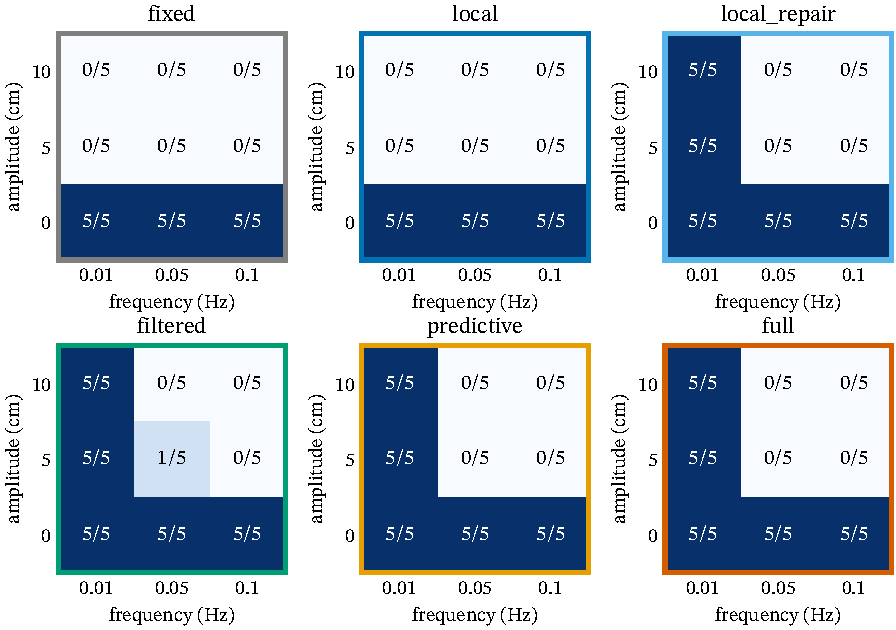
\includegraphics[width=0.9\linewidth]{figures/mulder/v1_pilot_completion}
\caption{Model v1 pilot: completed trials out of 5 for each policy, peak amplitude and forcing frequency
(endpoint executor). Wilson 95\% intervals are $[0.57,1]$ for 5/5, $[0.04,0.62]$ for 1/5 and $[0,0.43]$
for 0/5. $n=5$ seeds per cell, 270 trials. Source: \texttt{mulder\_\allowbreak{}results/\allowbreak{}pilot/\allowbreak{}trials.csv}.}
\label{fig:mulder-pilot-completion}
\end{figure}

\begin{figure}[htbp]
\centering
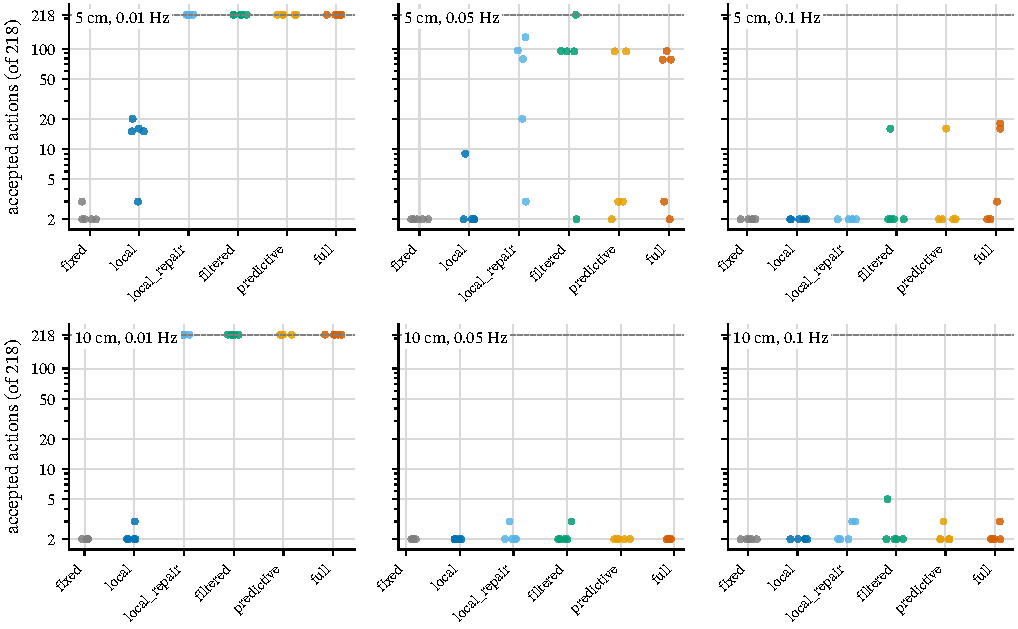
\includegraphics[width=\linewidth]{figures/mulder/v1_pilot_progress}
\caption{Model v1 pilot: accepted actions (of 218, log scale) per moving trial; dashed line is a complete
web. $n=5$ per policy and condition. Source: \texttt{mulder\_\allowbreak{}results/\allowbreak{}pilot/\allowbreak{}trials.csv}.}
\label{fig:mulder-pilot-progress}
\end{figure}

Among completed 0.01\,Hz webs, construction took longer than the stationary 1476.6\,s and grew with
amplitude (Figure~\ref{fig:mulder-pilot-costs}). In this v1 endpoint setting \texttt{full} was the fastest
completing policy (mean 1596.5\,s at 5\,cm, 1742.7\,s at 10\,cm, against 1703.2 and 1904.5\,s for
\texttt{local\_\allowbreak{}repair}) and travelled least (1.11 and 1.20 times the ideal static path), but it did so with
225 and 277 repairs per trial, about 0.94--1.12\,s of planning wall time, and the largest planning
counts. This v1 observation predates the audit fixes and concerns the endpoint executor at a frequency
outside the paper's; it does not carry over to the v3 primary comparison (Section~\ref{sec:mulder-v3}).

\begin{figure}[htbp]
\centering
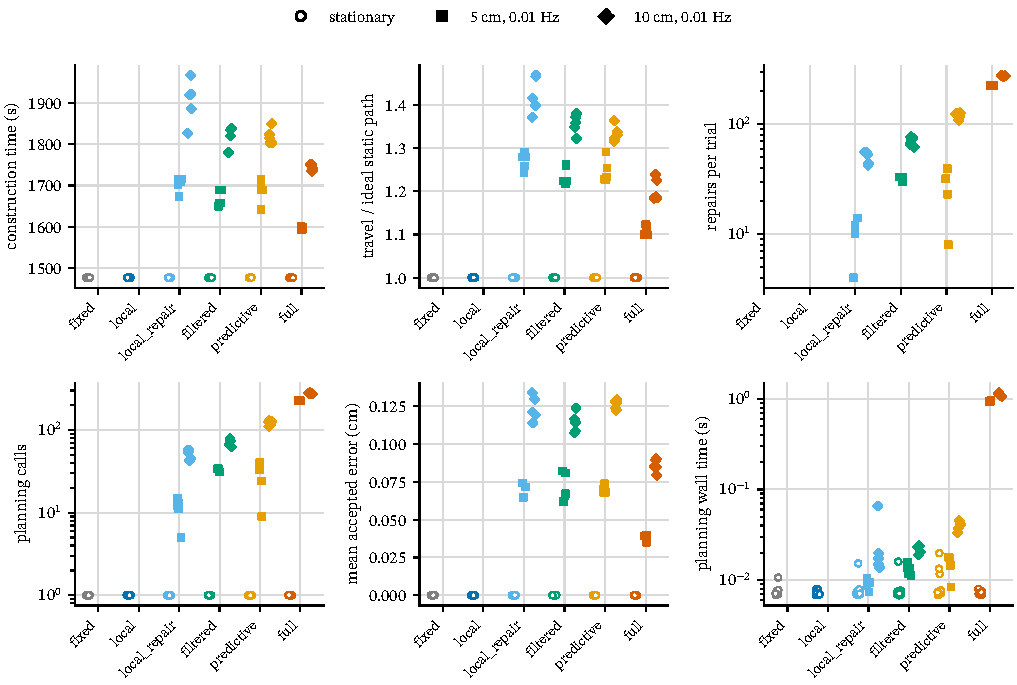
\includegraphics[width=\linewidth]{figures/mulder/v1_pilot_costs}
\caption{Model v1 pilot: per-trial costs of completed webs. Open circles: stationary runs (15 per policy:
three frequencies $\times$ five seeds, identical runs); squares and diamonds: completed runs at 0.01\,Hz with
5 and 10\,cm amplitude ($n=5$ each; \texttt{fixed} and \texttt{local} never completed). Repairs and planning
calls on log scales (zeros omitted). Source: \texttt{mulder\_\allowbreak{}results/\allowbreak{}pilot/\allowbreak{}trials.csv}.}
\label{fig:mulder-pilot-costs}
\end{figure}

The pilot is the only study with per-trial traces in usable numbers. Each
\texttt{trace\_\allowbreak{}<case>\_\allowbreak{}<seed>\_\allowbreak{}<policy>.json} records every attempt (start and end in material coordinates,
error, acceptance, phase, time) and every repair; \texttt{<case>} enumerates amplitude (outer loop) and
frequency in the order of \texttt{metadata.json}, so case 6 is 10\,cm/0.01\,Hz and case 4 is 5\,cm/0.05\,Hz.
Figure~\ref{fig:mulder-webs} draws the accepted silk of seed~0 for all six policies under the two
conditions, Figure~\ref{fig:mulder-timeseries} shows the same trials over time, and
Figure~\ref{fig:mulder-snapshots} replaces the material-coordinate view with the room-frame geometry of
one completed web at four times. The repository's own SVG drawings of the same traces are collected in
Figures~\ref{fig:mulder-gallery-a5}--\ref{fig:mulder-gallery-a10} (all five seeds of the conditions in which
webs complete; the 0.1\,Hz and 10\,cm/0.05\,Hz drawings were not included because every panel shows at most
22 accepted actions and is nearly blank).

\begin{figure}[htbp]
\centering
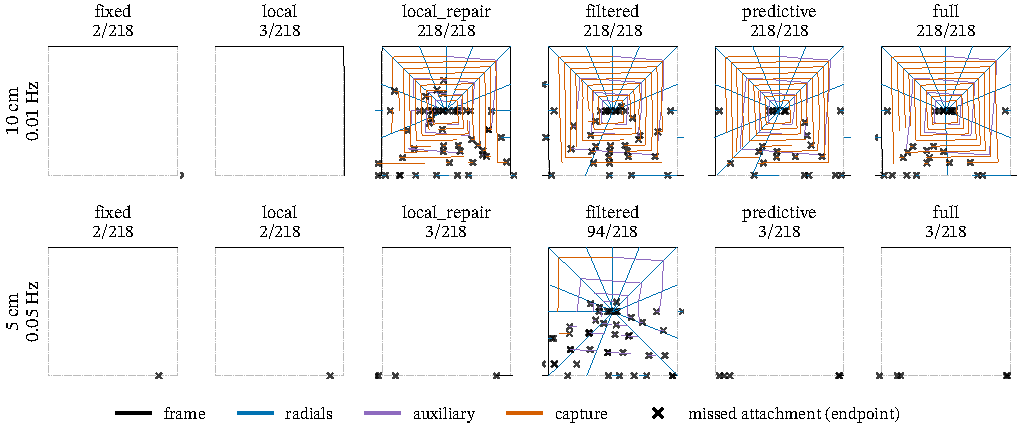
\includegraphics[width=\linewidth]{figures/mulder/v1_webs_six_policies}
\caption{Own drawing from model v1 pilot traces, seed~0: accepted silk chords in material coordinates
coloured by phase; crosses mark the end points of missed attempts. Top: 10\,cm, 0.01\,Hz (four policies
complete). Bottom: 5\,cm, 0.05\,Hz (only \texttt{filtered} progresses, to 94 actions). A chord is drawn from
the agent's actual start position, which after a missed attempt can lie off the ideal geometry; the
drawing is a kinematic record, not a relaxed web. Sources:
\texttt{mulder\_\allowbreak{}results/\allowbreak{}pilot/\allowbreak{}trace\_\allowbreak{}6\_\allowbreak{}0\_\allowbreak{}<policy>.json}, \texttt{trace\_\allowbreak{}4\_\allowbreak{}0\_\allowbreak{}<policy>.json}.}
\label{fig:mulder-webs}
\end{figure}

\begin{figure}[htbp]
\centering
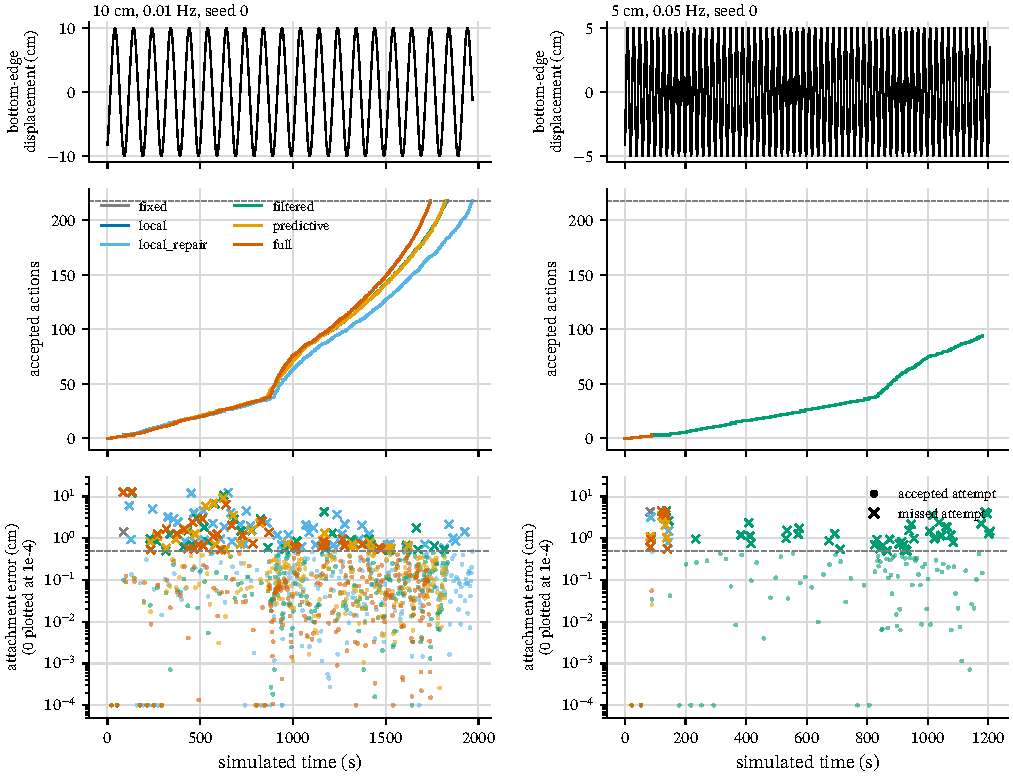
\includegraphics[width=\linewidth]{figures/mulder/v1_trial_timeseries}
\caption{Model v1 pilot, seed~0, the twelve trials of Figure~\ref{fig:mulder-webs}. Top: bottom-edge
displacement $A\sin(2\pi ft+\varphi)$ with $\varphi=5.306$\,rad from \texttt{trials.csv}. Middle: cumulative
accepted actions per policy. Bottom: final attachment error of every attempt (dots accepted, crosses
missed; dashed line is the 0.5\,cm tolerance; exact zeros plotted at $10^{-4}$). Source:
\texttt{mulder\_results/pilot/trace\_\{6,4\}\_0\_<policy>.json}.}
\label{fig:mulder-timeseries}
\end{figure}

\begin{figure}[htbp]
\centering
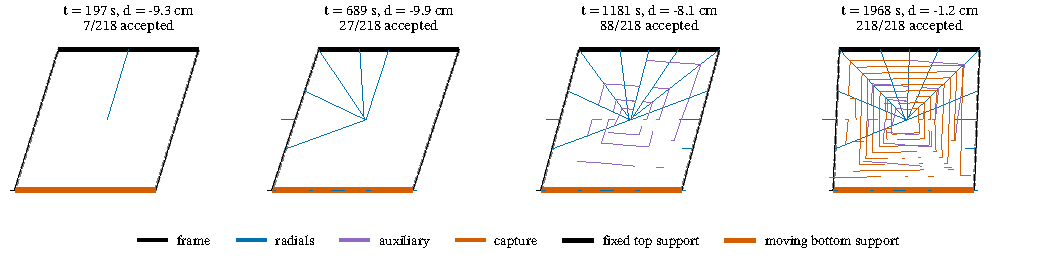
\includegraphics[width=\linewidth]{figures/mulder/v1_world_snapshots}
\caption{Own drawing: one completed model v1 web (\texttt{local\_\allowbreak{}repair}, 10\,cm, 0.01\,Hz, seed~0, 1967.5\,s)
in room coordinates at 10, 35, 60 and 100\% of its construction time. Threads accepted by time $t$ are
mapped through Eq.~\eqref{eq:mulder-shear}; $d$ is the bottom-edge displacement at $t$. This is the
affine kinematic map, not a mechanical deformation. Source:
\texttt{mulder\_\allowbreak{}results/\allowbreak{}pilot/\allowbreak{}trace\_\allowbreak{}6\_\allowbreak{}0\_\allowbreak{}local\_\allowbreak{}repair.json}.}
\label{fig:mulder-snapshots}
\end{figure}

\begin{figure}[p]
\centering
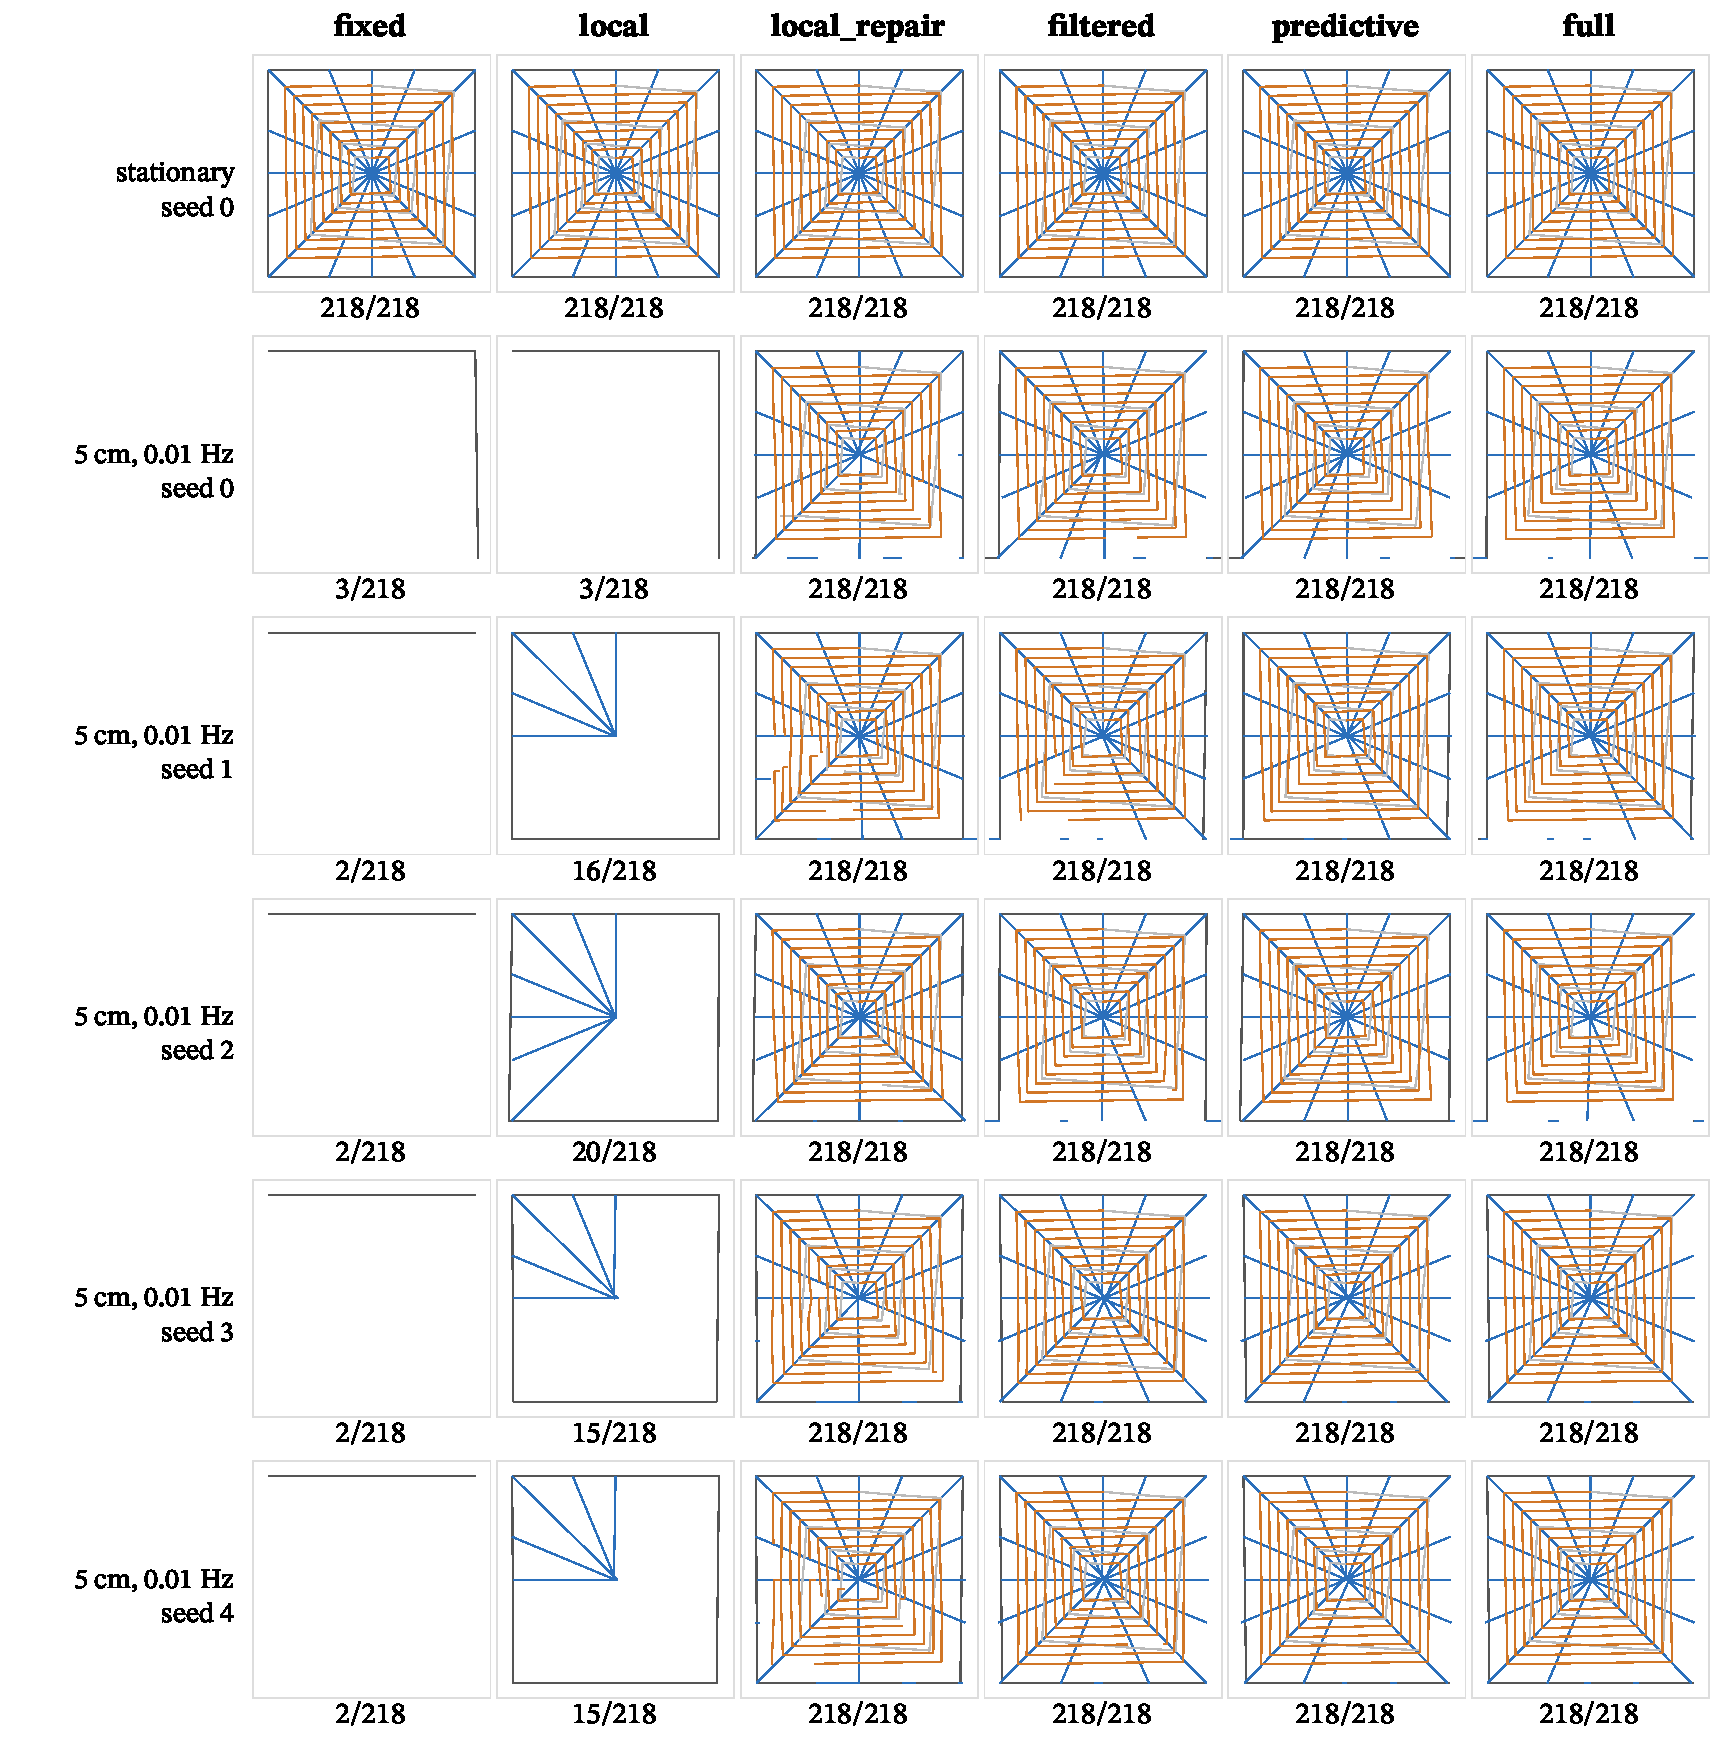
\includegraphics[width=\linewidth]{figures/mulder/gallery_v1_pilot_A5_f001}
\caption{The repository's own model v1 web drawings (\texttt{trace\_\allowbreak{}*.svg}), converted unchanged except for
a fixed 0.8\,px line width. Selection rule: stationary seed~0, then all five seeds at 5\,cm, 0.01\,Hz. Labels:
accepted actions from \texttt{trials.csv}. Repo colours: frame dark grey, radii blue, auxiliary light grey,
capture orange. Source: \texttt{mulder\_\allowbreak{}results/\allowbreak{}pilot/\allowbreak{}trace\_\allowbreak{}0\_\allowbreak{}0\_\allowbreak{}*.svg}, \texttt{trace\_\allowbreak{}3\_\allowbreak{}<seed>\_\allowbreak{}*.svg}.}
\label{fig:mulder-gallery-a5}
\end{figure}

\begin{figure}[p]
\centering
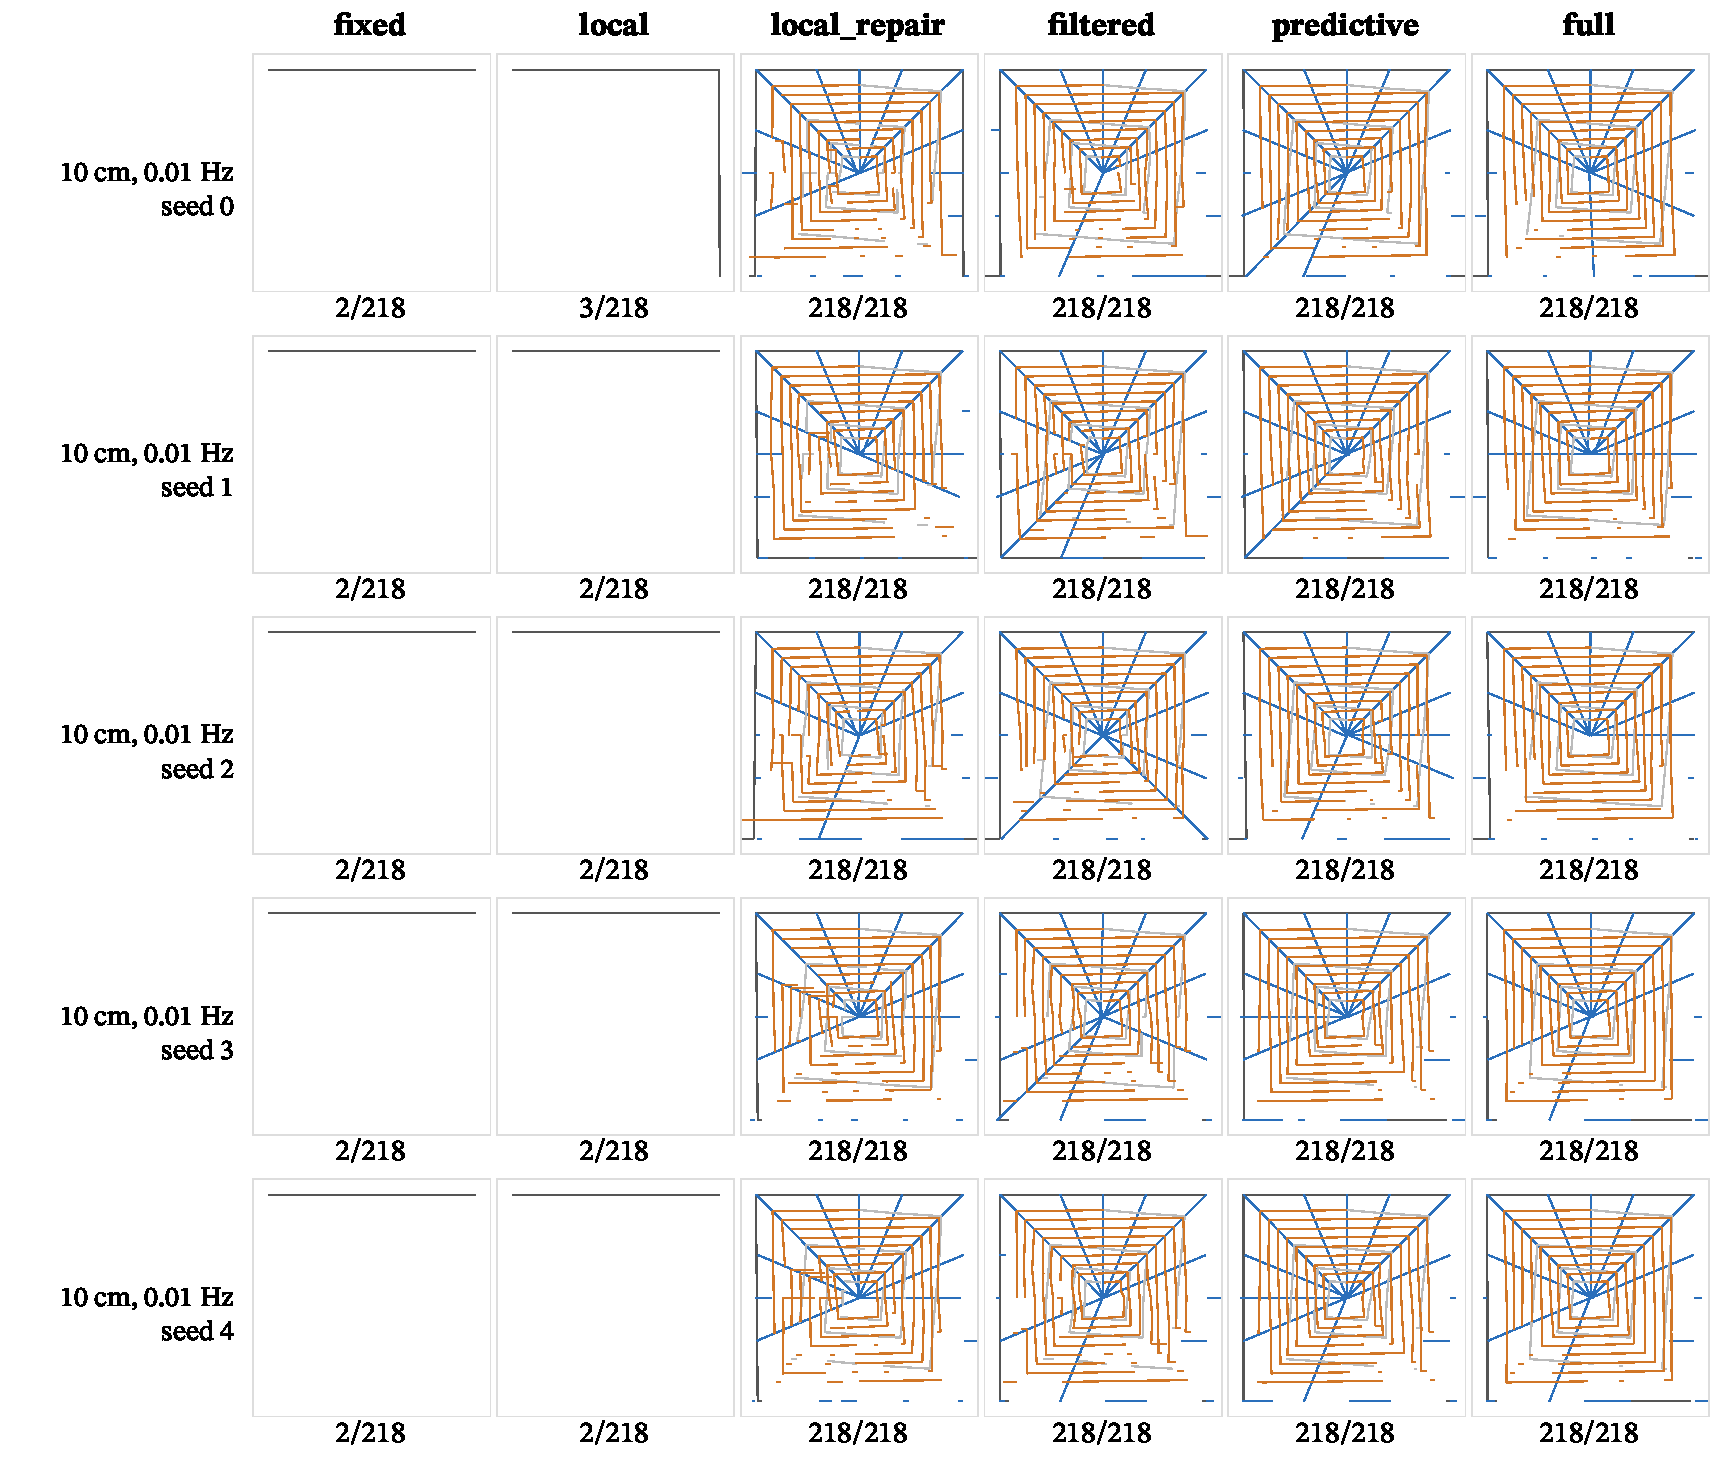
\includegraphics[width=\linewidth]{figures/mulder/gallery_v1_pilot_A10_f001}
\caption{As Figure~\ref{fig:mulder-gallery-a5}, all five seeds at 10\,cm, 0.01\,Hz (model v1). Source:
\texttt{mulder\_\allowbreak{}results/\allowbreak{}pilot/\allowbreak{}trace\_\allowbreak{}6\_\allowbreak{}<seed>\_\allowbreak{}*.svg}.}
\label{fig:mulder-gallery-a10}
\end{figure}

\subsubsection{Version 1 frequency study: 0.049 versus 0.05\,Hz}
\label{sec:mulder-freq}

Because the configured environment uses 0.049\,Hz and the paper about 0.05\,Hz, the v1 study repeated
the sweep at both frequencies (180 trials). All 60 stationary runs completed; of the 120 moving runs only
two completed (\texttt{full} at 5\,cm/0.049\,Hz and \texttt{filtered} at 5\,cm/0.05\,Hz), and at 10\,cm no
policy exceeded a mean of 5.4 accepted actions. Changing the frequency by 2\% did not produce a consistent
improvement for any policy: per-seed progress moved in both directions
(Figure~\ref{fig:mulder-freq}, left). The same comparison in v2 and in the v3 endpoint profile is shown
alongside. In v3 with 30 seeds the endpoint completions at 5\,cm were 0, 0, 0, 1, 1, 0 at 0.049\,Hz and
0, 0, 4, 3, 4, 0 at 0.05\,Hz (order \texttt{fixed}, \texttt{local}, \texttt{filtered}, \texttt{local\_\allowbreak{}repair},
\texttt{predictive}, \texttt{full}); under tracking every non-fixed policy completed 30/30 at both
frequencies, with duration changes that differ by at most 0.04 percentage points between frequencies
(Figure~\ref{fig:mulder-v3-paired}).

\begin{figure}[htbp]
\centering
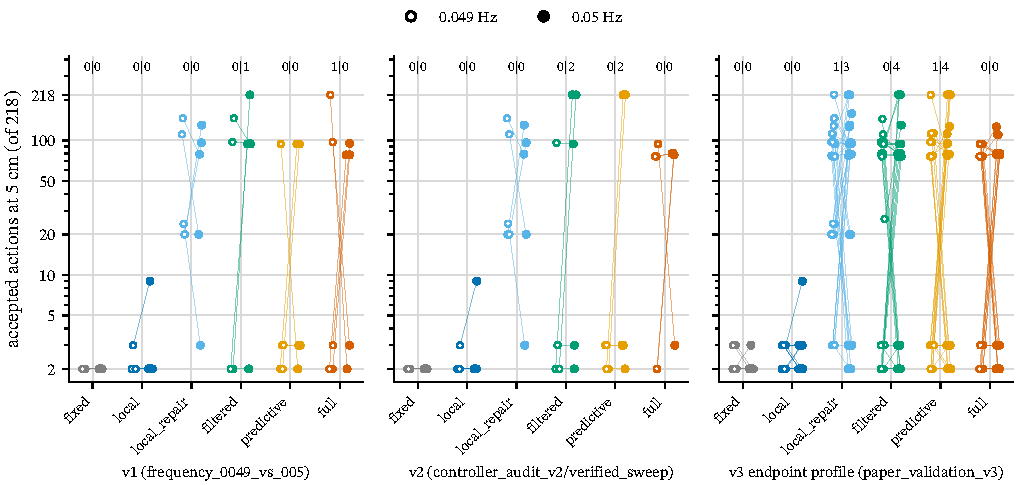
\includegraphics[width=\linewidth]{figures/mulder/freq_0049_vs_005}
\caption{Accepted actions at 5\,cm amplitude, 0.049\,Hz (open) versus 0.05\,Hz (filled); thin lines join the
same seed (same initial phase). Numbers above each policy: completions at 0.049\,|\,0.05\,Hz. Left: model v1
($n=5$ per point set), \texttt{mulder\_\allowbreak{}results/\allowbreak{}frequency\_\allowbreak{}0049\_\allowbreak{}vs\_\allowbreak{}005/\allowbreak{}trials.csv}. Middle: model v2
($n=5$), \texttt{controller\_\allowbreak{}audit\_\allowbreak{}v2/\allowbreak{}verified\_\allowbreak{}sweep/\allowbreak{}trials.csv}. Right: model v3 endpoint profile
($n=30$), \texttt{paper\_\allowbreak{}validation\_\allowbreak{}v3/\allowbreak{}trials.csv}. Versions are shown side by side, not pooled.}
\label{fig:mulder-freq}
\end{figure}

\begin{figure}[p]
\centering
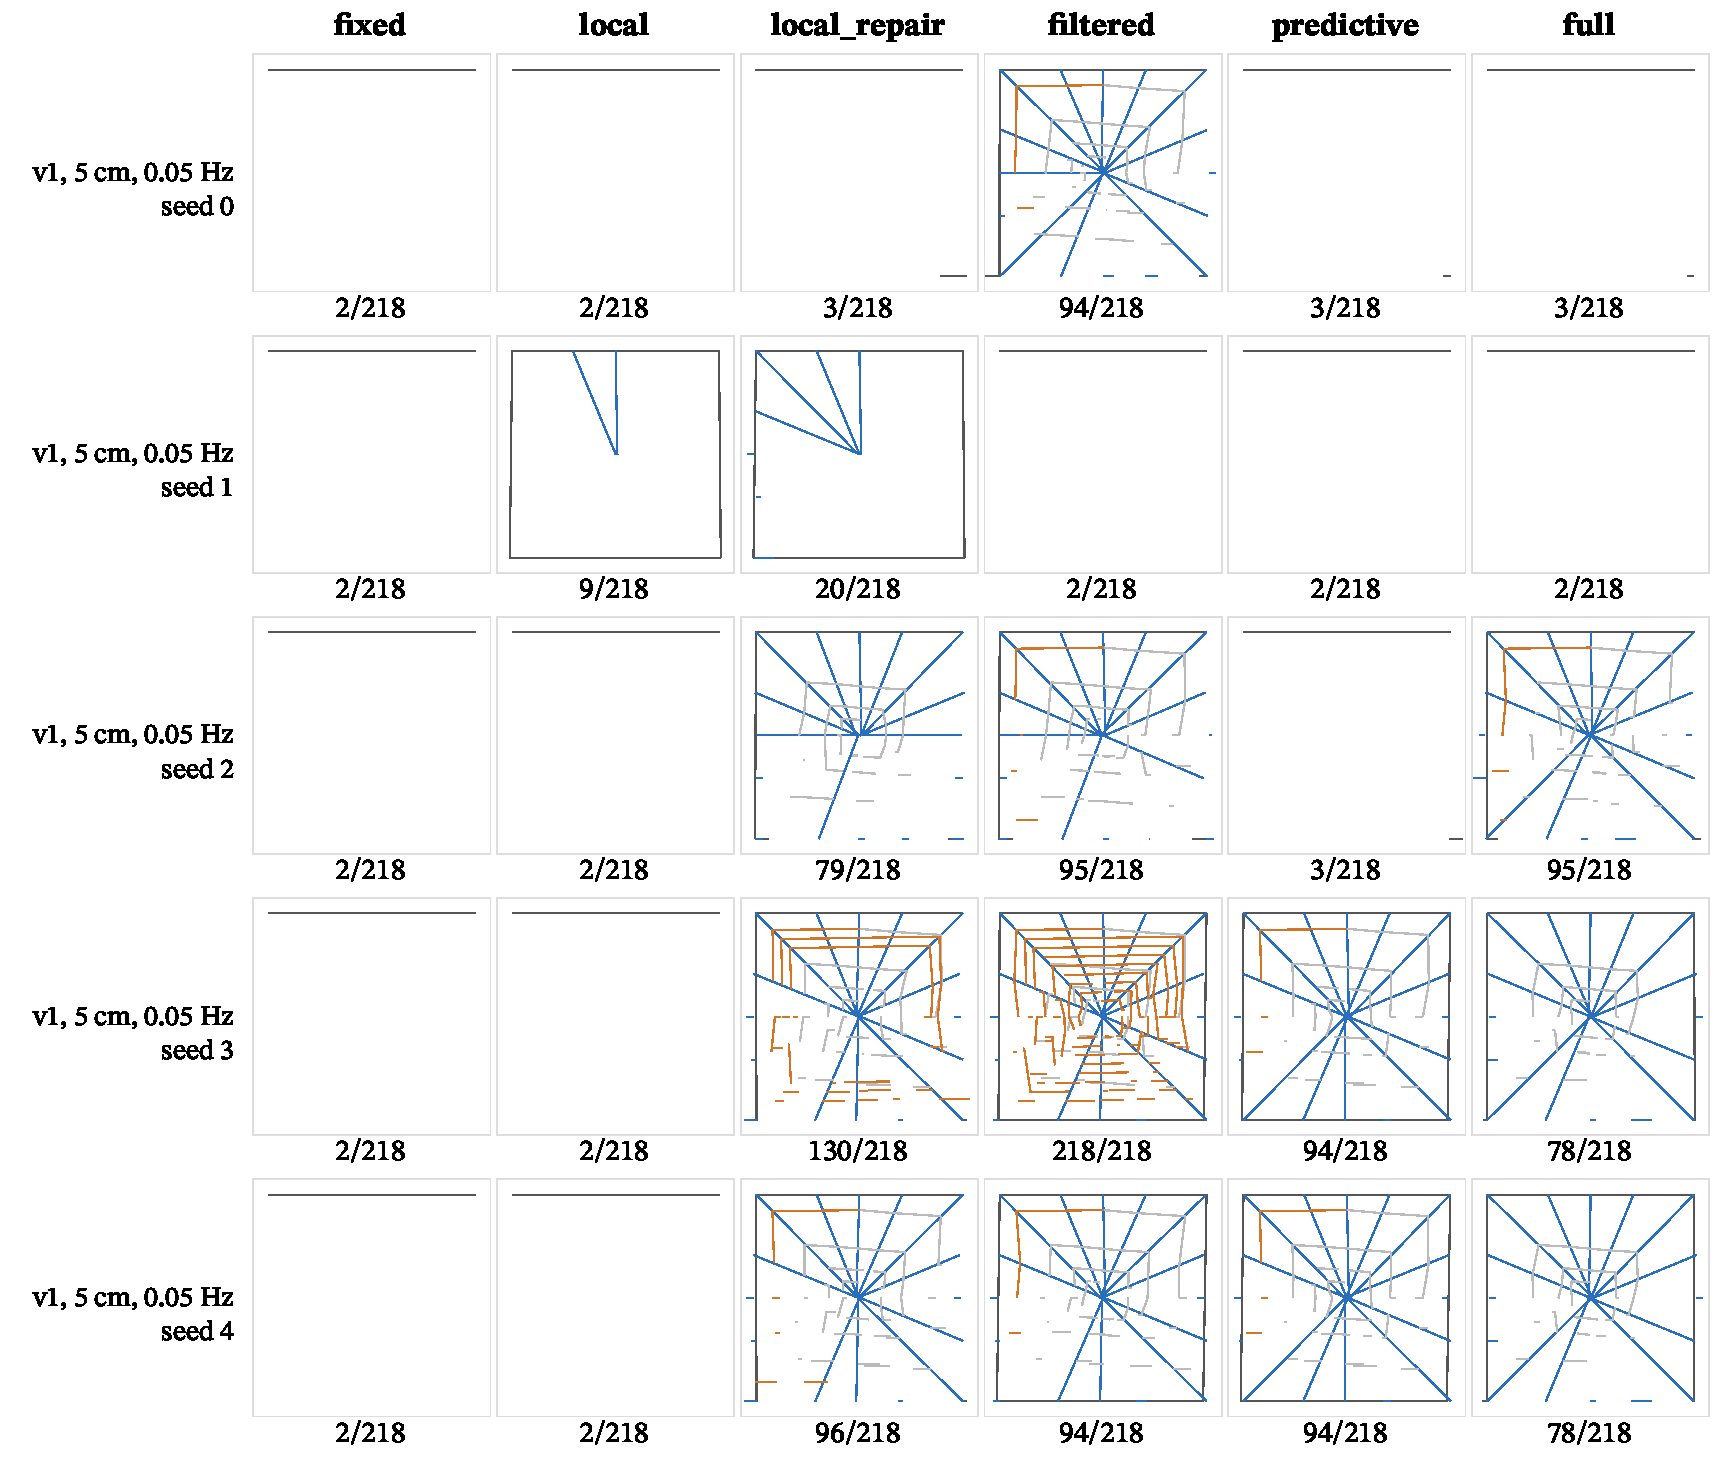
\includegraphics[width=\linewidth]{figures/mulder/gallery_v1_A5_f005}
\caption{Repository web drawings, model v1 frequency study, all five seeds at 5\,cm, 0.05\,Hz (converted as in
Figure~\ref{fig:mulder-gallery-a5}). Near-blank panels are failures at action 2--3. Source:
\texttt{mulder\_\allowbreak{}results/\allowbreak{}frequency\_\allowbreak{}0049\_\allowbreak{}vs\_\allowbreak{}005/\allowbreak{}trace\_\allowbreak{}3\_\allowbreak{}<seed>\_\allowbreak{}*.svg}.}
\label{fig:mulder-gallery-v1}
\end{figure}

\subsubsection{Version 2 controller audit}
\label{sec:mulder-audit}

An audit then checked whether each policy actually followed its stated rule, and found four defects
(\texttt{CONTROLLER\_\allowbreak{}AUDIT.md}): (i) \texttt{full} compared only the frame displacement at two action
boundaries and could miss a complete intervening cycle; (ii) a reactive retry could be followed by a
redundant proactive refresh; (iii) the \texttt{filtered} estimate mixed drift from unrelated components;
(iv) policy capabilities were scattered through name comparisons. All four were corrected, and the
v1 outputs were preserved and labelled as v1.

\paragraph{Matched diagnostic.} One matched trial per policy (5\,cm, 0.05\,Hz, seed~0) was recorded with a
complete event ledger (41 attempts, 41 decisions, 26 repairs), an intended-versus-attempted action map and
isolated replays of each policy's first miss. All six policies failed at segment~2 or~3, the first frame
edges reaching the moving bottom (Figures~\ref{fig:mulder-audit-attempts}--\ref{fig:mulder-audit-errors});
the action map shows no policy reached segment~4. \texttt{fixed} and \texttt{local} stopped at 2/218;
\texttt{local\_\allowbreak{}repair} (4 repairs), \texttt{filtered} and \texttt{predictive} (7 each) and \texttt{full}
(8) reached 3/218. The replays (Figure~\ref{fig:mulder-audit-replays}) separate two explanations. Refreshing
the target at departure alone never rescued the attempt, whereas freezing the frame after a refresh
always did, and a correction aimed with perfect knowledge of the future motion (``arrival oracle'') did
for every policy once the target was refreshed. The repository's reading, which we adopt, is that the
failures implicate the endpoint \emph{execution rule}, not only stale targets. The oracles are diagnostic
interventions; a failed oracle search is not a proof of physical unreachability.

\begin{figure}[htbp]
\centering
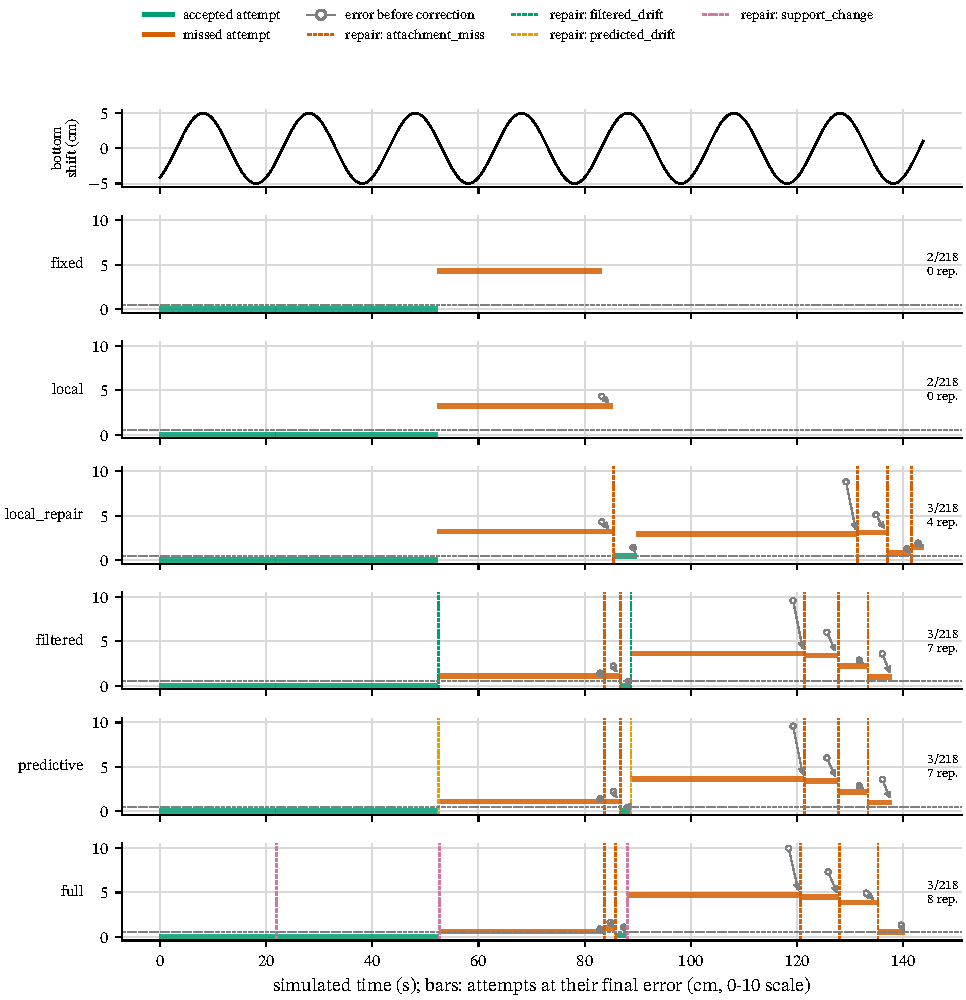
\includegraphics[width=\linewidth]{figures/mulder/audit_v2_attempts}
\caption{Model v2 matched diagnostic trial (endpoint executor, 5\,cm, 0.05\,Hz, seed~0). Top: bottom-edge
displacement. Below, one row per policy: each attempt as a bar spanning its duration at the height of its
final error (green accepted, vermillion missed); open circles and arrows show the error before the
endpoint correction; dashed verticals are repairs coloured by reason. Right: accepted actions and repairs.
Source: \texttt{mulder\_\allowbreak{}results/\allowbreak{}controller\_\allowbreak{}audit\_\allowbreak{}v2/\allowbreak{}report/\allowbreak{}ledger.csv}, \texttt{trials.csv}.}
\label{fig:mulder-audit-attempts}
\end{figure}

\begin{figure}[htbp]
\centering
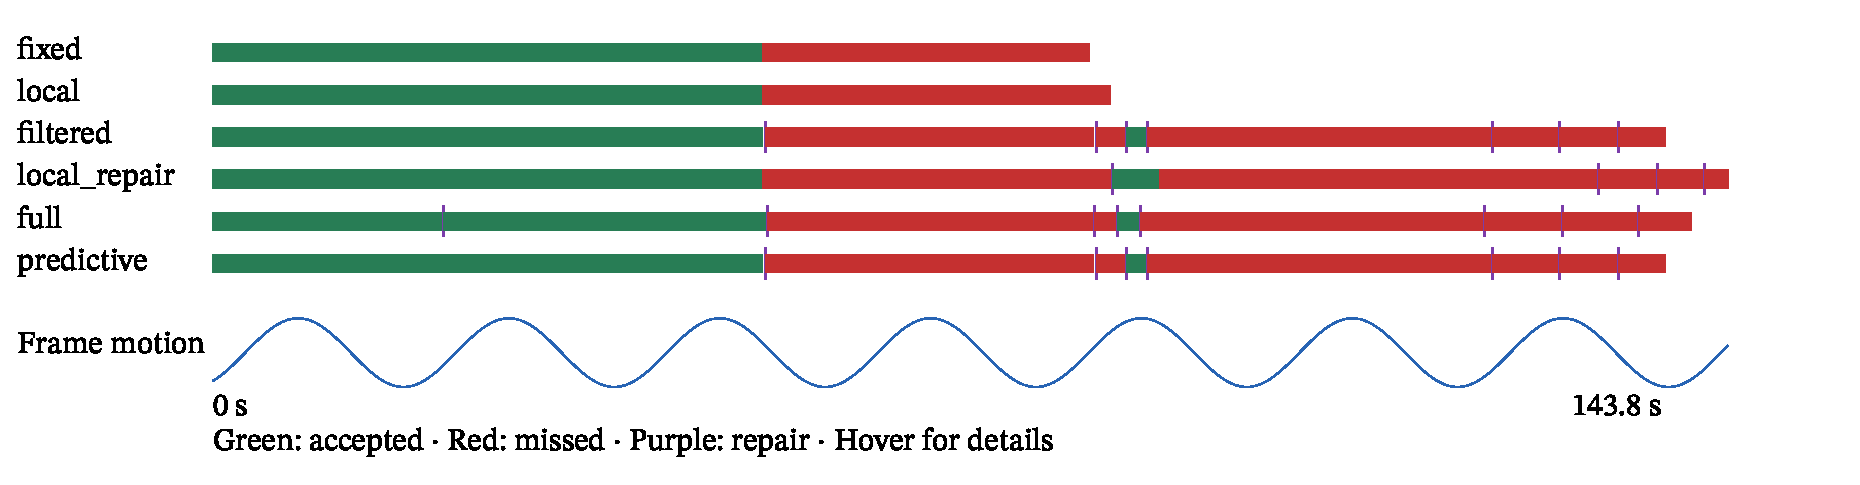
\includegraphics[width=\linewidth]{figures/mulder/audit_v2_timeline_repo}
\caption{The repository's own controller timeline for the same six trials (model v2):
\texttt{timeline.svg}, converted with its text enlarged for print and otherwise unchanged (green accepted,
red missed, purple repair; frame motion below; 0--143.8\,s). Source:
\texttt{mulder\_\allowbreak{}results/\allowbreak{}controller\_\allowbreak{}audit\_\allowbreak{}v2/\allowbreak{}report/\allowbreak{}timeline.svg}.}
\label{fig:mulder-audit-timeline}
\end{figure}

\begin{figure}[p]
\centering
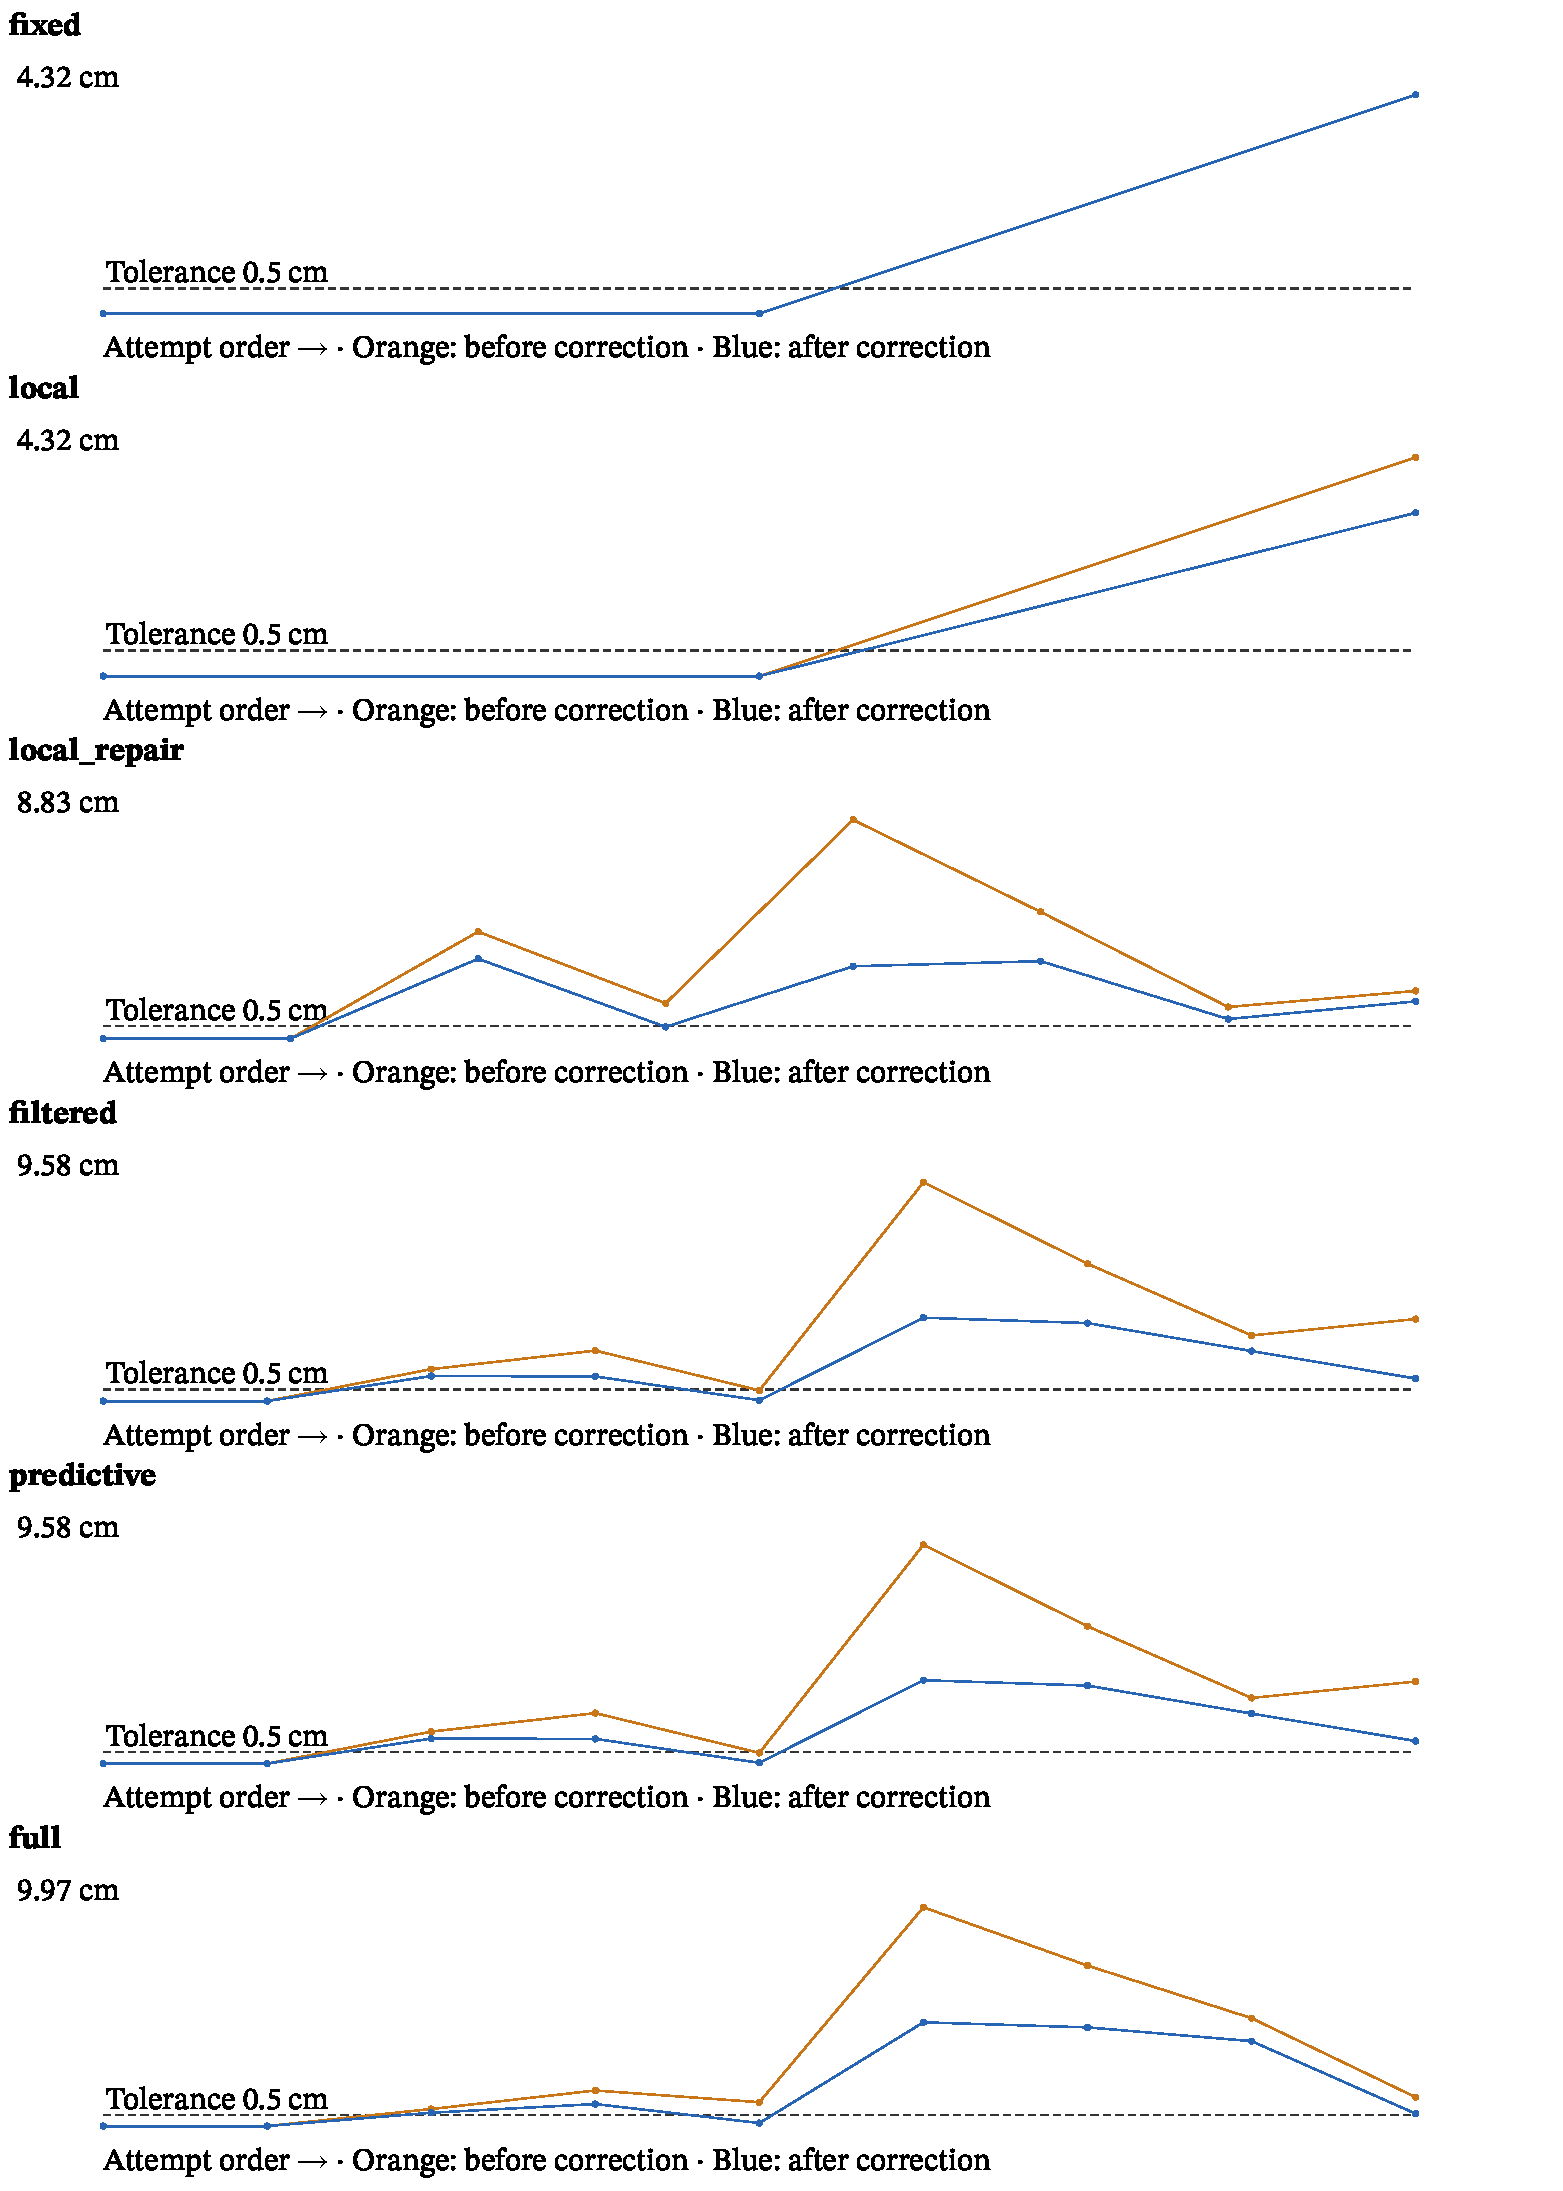
\includegraphics[width=0.8\linewidth]{figures/mulder/audit_v2_errors_repo}
\caption{The repository's own per-policy audit drawings \texttt{errors\_\allowbreak{}<policy>.svg} for the same six
trials (model v2), converted with enlarged text: attachment error by attempt order (orange before, blue
after the endpoint correction; dashed 0.5\,cm tolerance; vertical scale set by each plot's maximum, printed
at top left). Source: \texttt{mulder\_\allowbreak{}results/\allowbreak{}controller\_\allowbreak{}audit\_\allowbreak{}v2/\allowbreak{}report/\allowbreak{}}. The accompanying
\texttt{web\_\allowbreak{}<policy>.svg} drawings contain one or two threads each and are not reproduced.}
\label{fig:mulder-audit-errors}
\end{figure}

\begin{figure}[htbp]
\centering
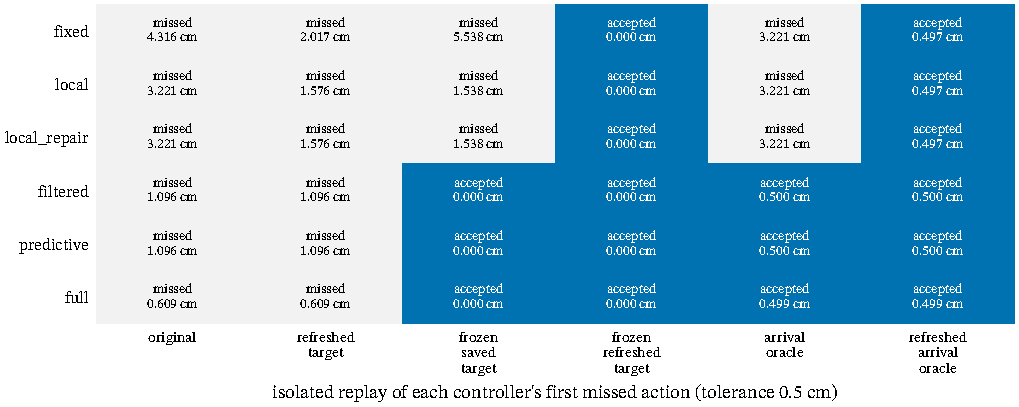
\includegraphics[width=\linewidth]{figures/mulder/audit_v2_replays}
\caption{Model v2 isolated replays of each policy's first missed action from the same start position and
time, without repair delay: \emph{original} (must reproduce the recorded miss); \emph{refreshed target} at
departure; \emph{frozen} frame with the saved or refreshed target; \emph{arrival oracle} corrections using
perfect future forcing, with the saved or refreshed target. Cells give acceptance and final error.
$n=36$ replays. Source: \texttt{mulder\_\allowbreak{}results/\allowbreak{}controller\_\allowbreak{}audit\_\allowbreak{}v2/\allowbreak{}report/\allowbreak{}replays.csv}.}
\label{fig:mulder-audit-replays}
\end{figure}

\paragraph{Verified sweep.} Re-running the 180-trial frequency comparison with the corrected
controllers gave 64 completions (all 60 stationary, plus \texttt{filtered} and \texttt{predictive} 2/5 each
at 5\,cm/0.05\,Hz), against 62 in v1. Per-seed progress was unchanged for \texttt{fixed}, \texttt{local} and
\texttt{local\_\allowbreak{}repair}, as expected, but moved substantially in both directions for the three proactive
policies (Figure~\ref{fig:mulder-v1v2}); for example \texttt{full} at 5\,cm/0.049\,Hz, seed~1 went from a
complete web (v1) to 76 actions (v2). With five seeds and endpoint execution still failing almost
everywhere, the audit changed which policy happened to survive individual phases rather than the overall
picture. At that stage 98 tests passed (work log).

\begin{figure}[htbp]
\centering
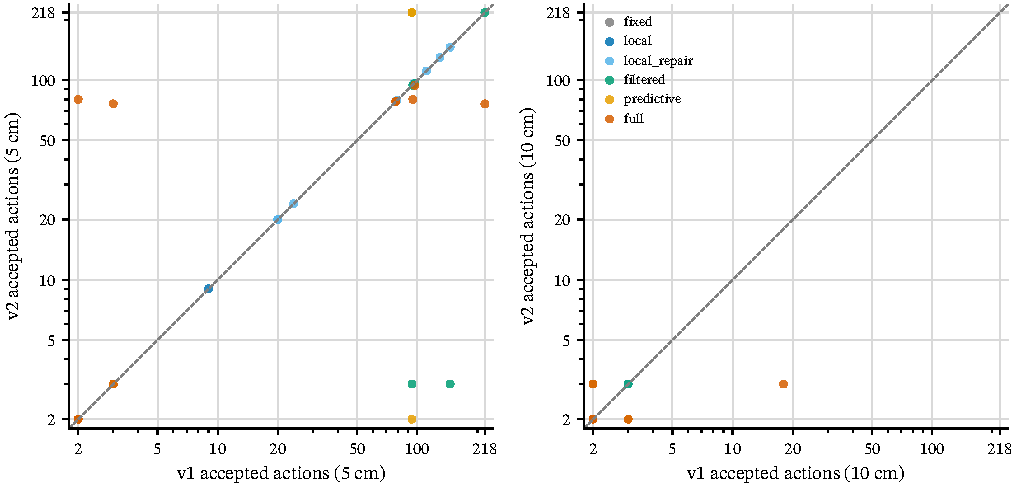
\includegraphics[width=0.95\linewidth]{figures/mulder/v1_vs_v2_progress}
\caption{Same seed and condition before (model v1) and after (model v2) the controller audit: accepted
actions per moving trial at 5\,cm (left) and 10\,cm (right), both frequencies; dashed line is no change.
$n=60$ trials per panel (overlapping points coincide). Sources:
\texttt{mulder\_\allowbreak{}results/\allowbreak{}frequency\_\allowbreak{}0049\_\allowbreak{}vs\_\allowbreak{}005/\allowbreak{}trials.csv},
\texttt{mulder\_\allowbreak{}results/\allowbreak{}controller\_\allowbreak{}audit\_\allowbreak{}v2/\allowbreak{}verified\_\allowbreak{}sweep/\allowbreak{}trials.csv}.}
\label{fig:mulder-v1v2}
\end{figure}

\begin{figure}[p]
\centering
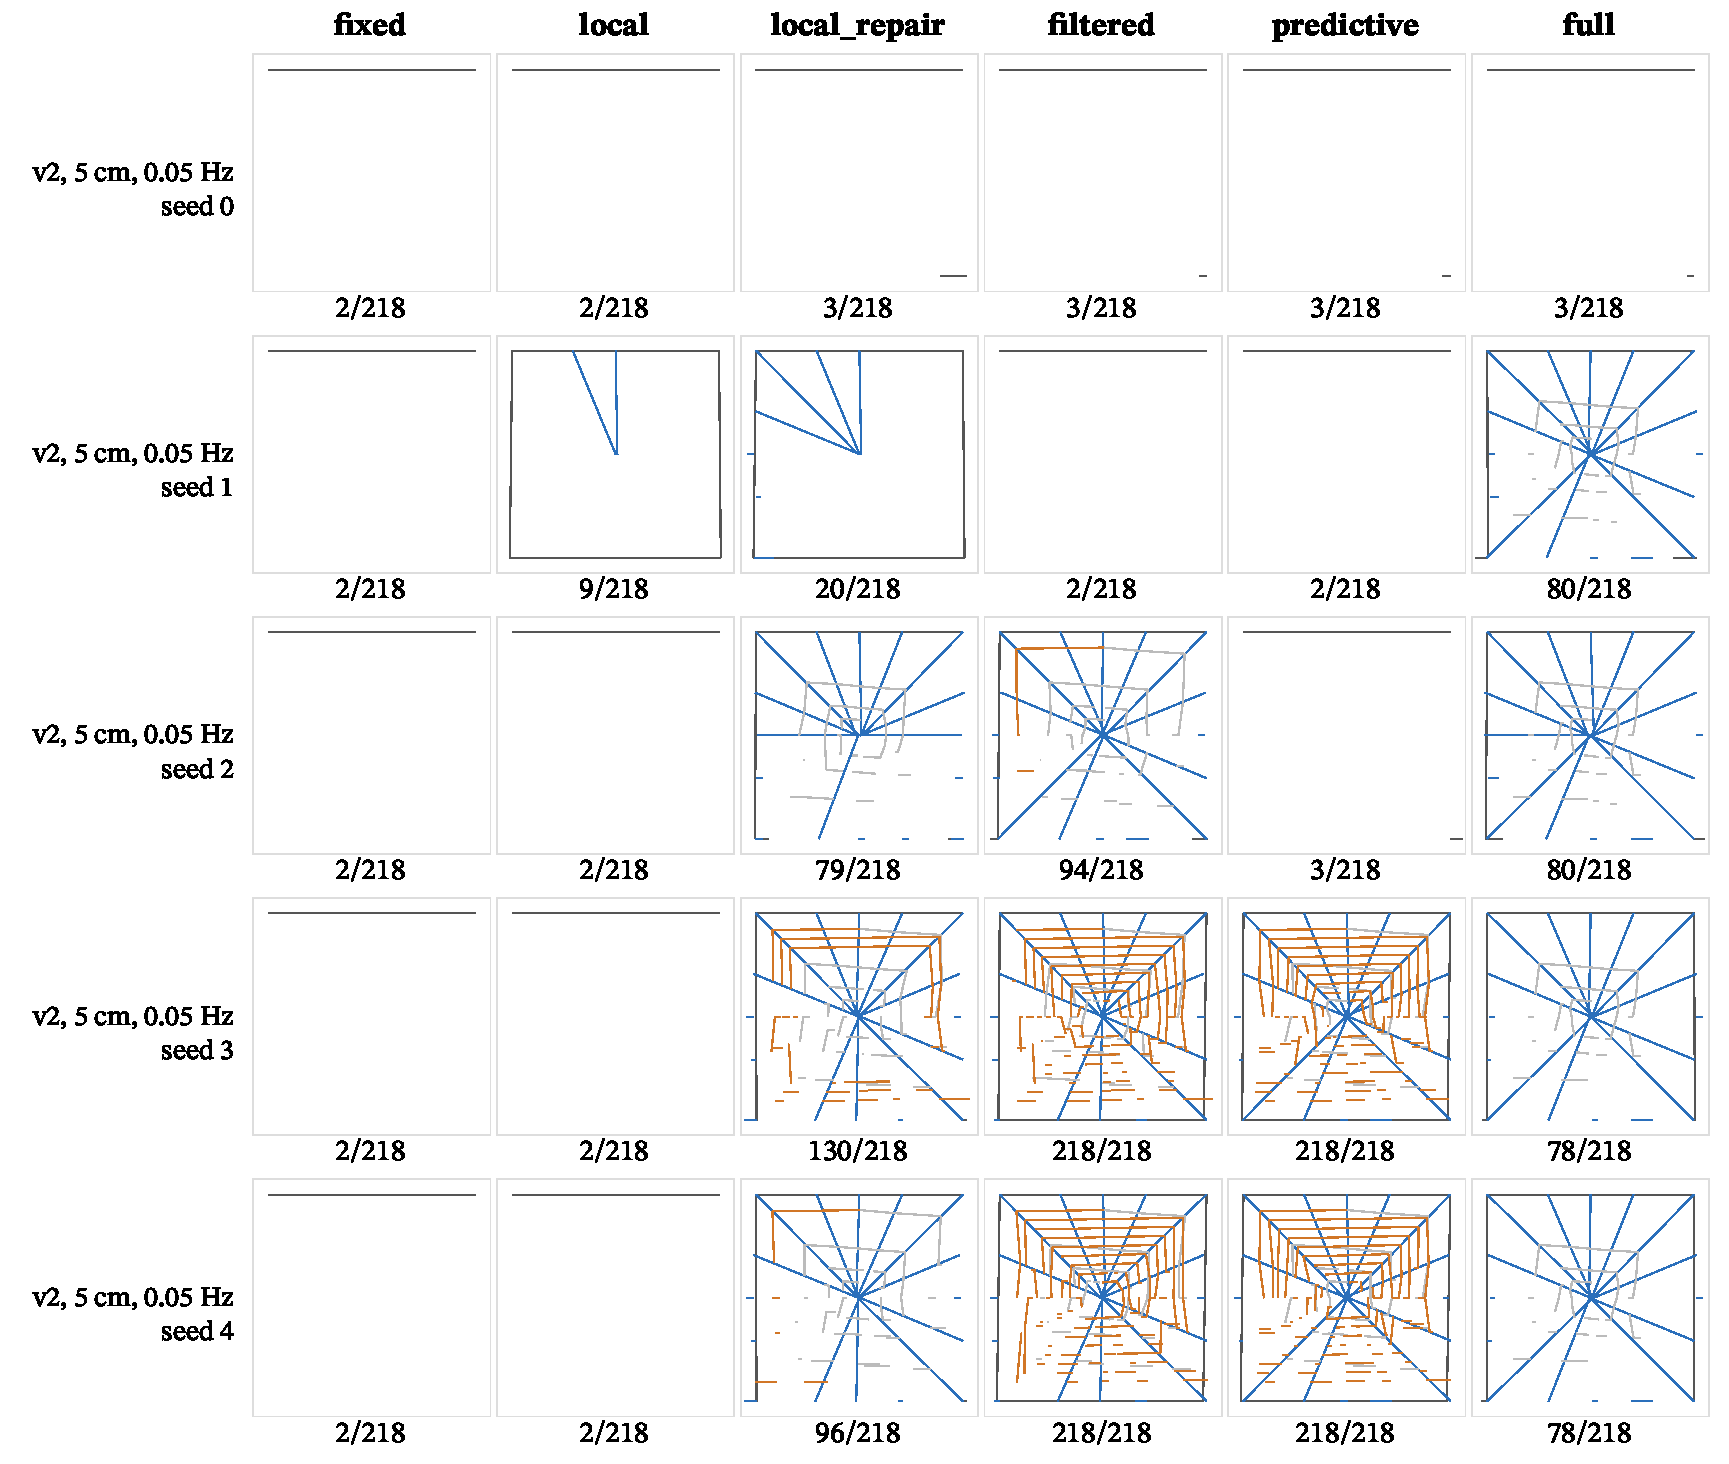
\includegraphics[width=\linewidth]{figures/mulder/gallery_v2_A5_f005}
\caption{Repository web drawings, model v2 verified sweep, all five seeds at 5\,cm, 0.05\,Hz (compare
Figure~\ref{fig:mulder-gallery-v1}, same seeds in v1). Source:
\texttt{mulder\_\allowbreak{}results/\allowbreak{}controller\_\allowbreak{}audit\_\allowbreak{}v2/\allowbreak{}verified\_\allowbreak{}sweep/\allowbreak{}trace\_\allowbreak{}3\_\allowbreak{}<seed>\_\allowbreak{}*.svg}.}
\label{fig:mulder-gallery-v2}
\end{figure}

\subsubsection{Version 3 paper-facing validation}
\label{sec:mulder-v3}

\paragraph{Completion.} Figures~\ref{fig:mulder-v3-completion-repo}--\ref{fig:mulder-v3-wilson} give
completion for the 1{,}800 primary trials. Under endpoint execution no policy completed any of 30 trials
at 10\,cm (C02), and at 5\,cm at most 4/30 (\texttt{filtered} and \texttt{predictive} at 0.05\,Hz; Wilson
$[0.053,0.297]$). Partial progress under endpoint execution at 5\,cm was bimodal: of 360 trials, 218 stopped within the first
three actions, 118 reached 75--149 actions and 13 completed (Figure~\ref{fig:mulder-endpoint-progress}).
Under ideal continuous tracking all five feedback policies completed 30/30 in every moving condition
(Wilson $[0.8865,1]$; C03), while \texttt{fixed} completed none (118 attachment misses and 2 action
deadlines in 120 moving trials). The ledger's interpretation is precise: C02 is a failure of that executor
and model, not physical impossibility or a failure of HTN planning generally, and C03 holds over initial
phases under assumed no-slip advection and ideal sensing.

\begin{figure}[htbp]
\centering
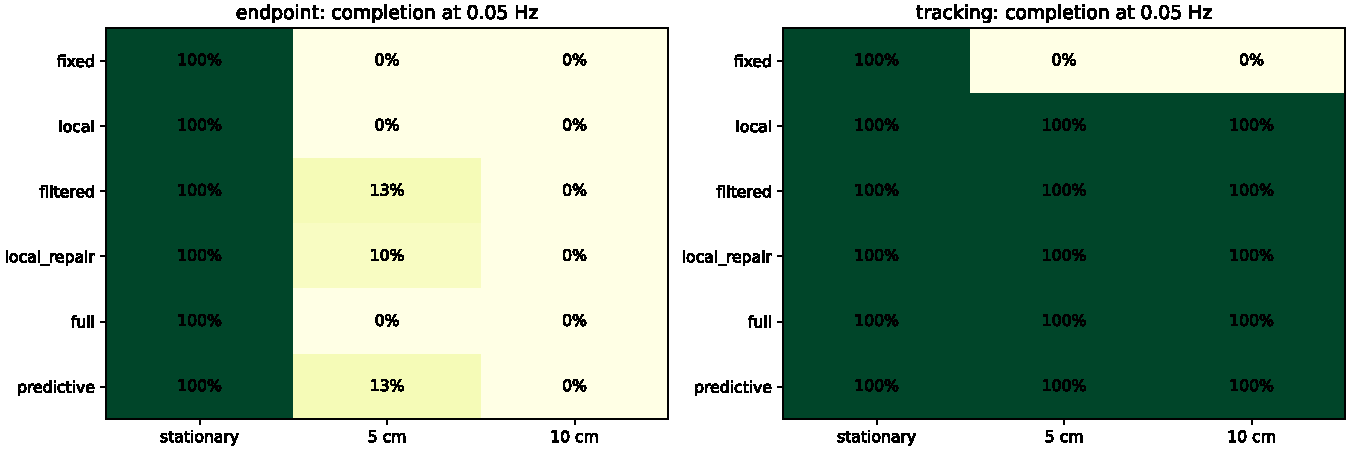
\includegraphics[width=\linewidth]{figures/mulder/repo_v3_completion}
\caption{The repository's manuscript figure \texttt{docs/\allowbreak{}manuscript/\allowbreak{}figures/\allowbreak{}mulder\_\allowbreak{}v3\_\allowbreak{}completion.svg}
(model v3), converted unchanged: completion at 0.05\,Hz by executor and policy; 30 initial phases per cell.}
\label{fig:mulder-v3-completion-repo}
\end{figure}

\begin{figure}[htbp]
\centering
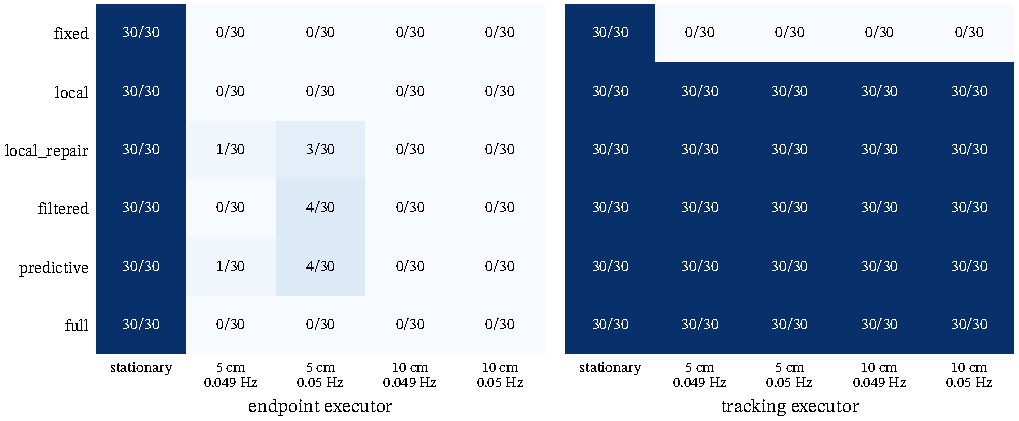
\includegraphics[width=\linewidth]{figures/mulder/v3_completion}
\caption{Regenerated in the shared style and extended to both frequencies: model v3 completed trials out
of 30 per cell. Stationary controls are shared by both frequencies. Source:
\texttt{mulder\_\allowbreak{}results/\allowbreak{}paper\_\allowbreak{}validation\_\allowbreak{}v3/\allowbreak{}trials.csv}.}
\label{fig:mulder-v3-completion}
\end{figure}

\begin{figure}[htbp]
\centering
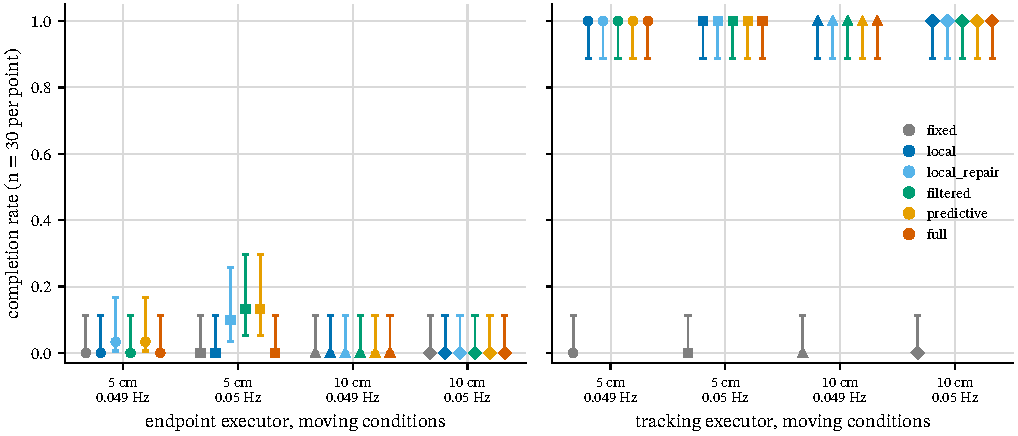
\includegraphics[width=\linewidth]{figures/mulder/v3_completion_wilson}
\caption{Model v3 completion rates with Wilson 95\% intervals (Eq.~\ref{eq:mulder-wilson}), moving conditions;
$n=30$ per point. Marker shape encodes the condition. Source:
\texttt{mulder\_\allowbreak{}results/\allowbreak{}paper\_\allowbreak{}validation\_\allowbreak{}v3/\allowbreak{}trials.csv}.}
\label{fig:mulder-v3-wilson}
\end{figure}

\begin{figure}[htbp]
\centering
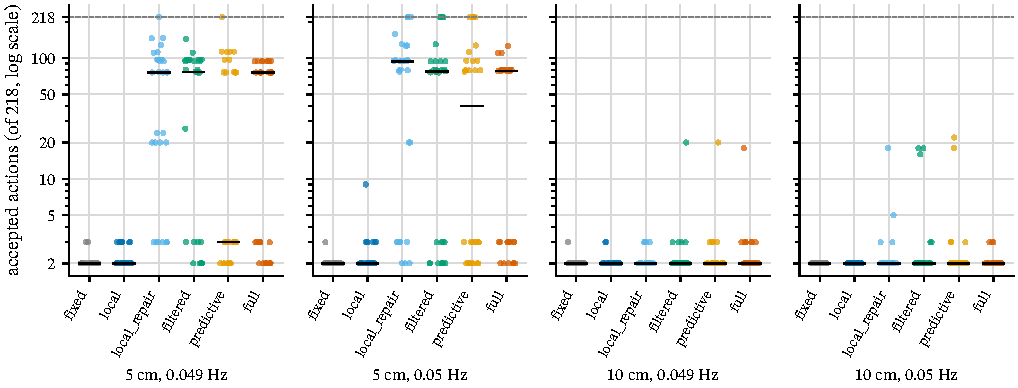
\includegraphics[width=\linewidth]{figures/mulder/v3_endpoint_progress}
\caption{Model v3 endpoint profile: accepted actions per trial (log scale; black bar = median; dashed line =
complete web). $n=30$ per policy and condition. Source: \texttt{mulder\_\allowbreak{}results/\allowbreak{}paper\_\allowbreak{}validation\_\allowbreak{}v3/\allowbreak{}trials.csv}.}
\label{fig:mulder-endpoint-progress}
\end{figure}

\paragraph{Paired moving--stationary effects.} Table~\ref{tab:mulder-v3-effects} and
Figures~\ref{fig:mulder-v3-paired-repo}--\ref{fig:mulder-v3-paired} report the paired contrasts for tracking.
For \texttt{local} at 10\,cm and 0.05\,Hz, construction took 1491.076902\,s under movement against
1476.595732\,s stationary, a paired increase of 0.980713\% (95\% interval 0.963429--0.996403\%); the
interval excludes zero, so the model does \emph{not} show identical time (C04 is unsupported) and must not be
described as replicating the paper's non-significant test (C05). \texttt{full} also completed every trial but
was slower, +3.923865\% (3.893372--3.953719\%). Camera-sampled travel for \texttt{local} rose by 1.130044\%
(1.079618--1.180734\%), whereas the true frame-relative travel was identical to within $10^{-13}$\,cm
(1367.595732\,cm), because under zero-lag tracking the material end points are imposed. At 5\,cm the
duration increase was smaller (+0.281\%) and sampled travel \emph{fell} by 0.927\% (0.946--0.909\%). The
time shares moved by fractions of a percentage point (Figure~\ref{fig:mulder-v3-phase}).
\texttt{local}, \texttt{local\_\allowbreak{}repair} and \texttt{predictive} produced identical trajectories: no repair or
proactive refresh was ever triggered under ideal tracking.

\begin{table}[htbp]
\centering
\small
\begin{tabular}{@{}l l r r r@{}}
\toprule
Policy & Outcome & Moving mean & Stationary mean & Paired change, \% [95\% CI] \\
\midrule
\texttt{local} & duration (s) & 1491.077 & 1476.596 & $+0.981$ [0.963, 0.996] \\
\texttt{local} & sampled travel (cm) & 1136.020 & 1123.326 & $+1.130$ [1.080, 1.181] \\
\texttt{local} & true travel (cm) & 1367.596 & 1367.596 & $0.000$ \\
\texttt{predictive} & duration (s) & 1491.077 & 1476.596 & $+0.981$ [0.964, 0.998] \\
\texttt{filtered} & duration (s) & 1508.839 & 1476.596 & $+2.184$ \\
\texttt{full} & duration (s) & 1534.535 & 1476.596 & $+3.924$ [3.893, 3.954] \\
\texttt{full} & sampled travel (cm) & 1141.120 & 1123.326 & $+1.584$ [1.473, 1.689] \\
\bottomrule
\end{tabular}
\caption{Model v3, tracking executor, 10\,cm, 0.05\,Hz: paired moving-minus-stationary contrasts over 30
completed pairs (paired bootstrap, 2{,}000 resamples). Source:
\texttt{mulder\_\allowbreak{}results/\allowbreak{}paper\_\allowbreak{}validation\_\allowbreak{}v3/\allowbreak{}comparisons.csv}; the \texttt{local} and \texttt{full} rows are also
recorded in \texttt{docs/\allowbreak{}research/\allowbreak{}evidence/\allowbreak{}mulder\_\allowbreak{}v3\_\allowbreak{}summary.json}.}
\label{tab:mulder-v3-effects}
\end{table}

\begin{figure}[htbp]
\centering
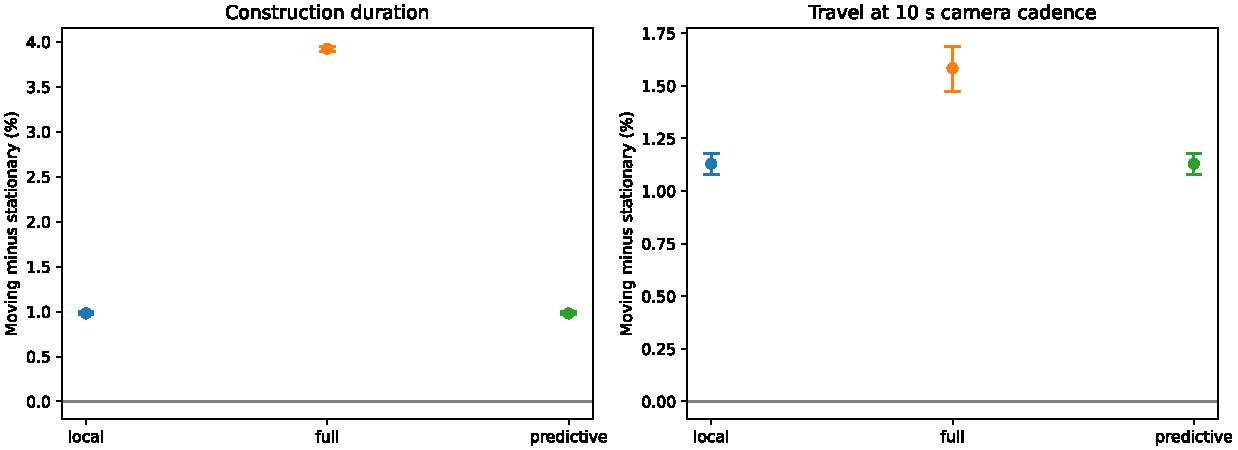
\includegraphics[width=\linewidth]{figures/mulder/repo_v3_paired_effects}
\caption{The repository's manuscript figure \texttt{docs/\allowbreak{}manuscript/\allowbreak{}figures/\allowbreak{}mulder\_\allowbreak{}v3\_\allowbreak{}paired\_\allowbreak{}effects.svg}
(model v3), converted unchanged: paired moving-minus-stationary change at 10\,cm, 0.05\,Hz, with 95\%
paired-bootstrap intervals over 30 forcing phases (local blue, full orange, predictive green in the repo's
colours).}
\label{fig:mulder-v3-paired-repo}
\end{figure}

\begin{figure}[htbp]
\centering
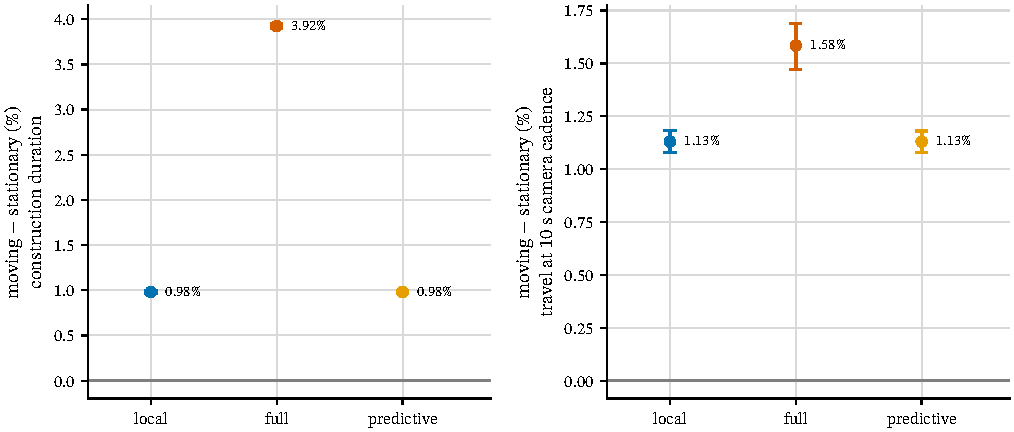
\includegraphics[width=\linewidth]{figures/mulder/v3_paired_effects_primary}
\caption{Shared-style regeneration of Figure~\ref{fig:mulder-v3-paired-repo} from
\texttt{mulder\_\allowbreak{}results/\allowbreak{}paper\_\allowbreak{}validation\_\allowbreak{}v3/\allowbreak{}comparisons.csv}: mean paired change with 95\% paired-bootstrap
interval; 30 pairs each (duration intervals are narrower than the markers).}
\label{fig:mulder-v3-paired-primary}
\end{figure}

\begin{figure}[htbp]
\centering
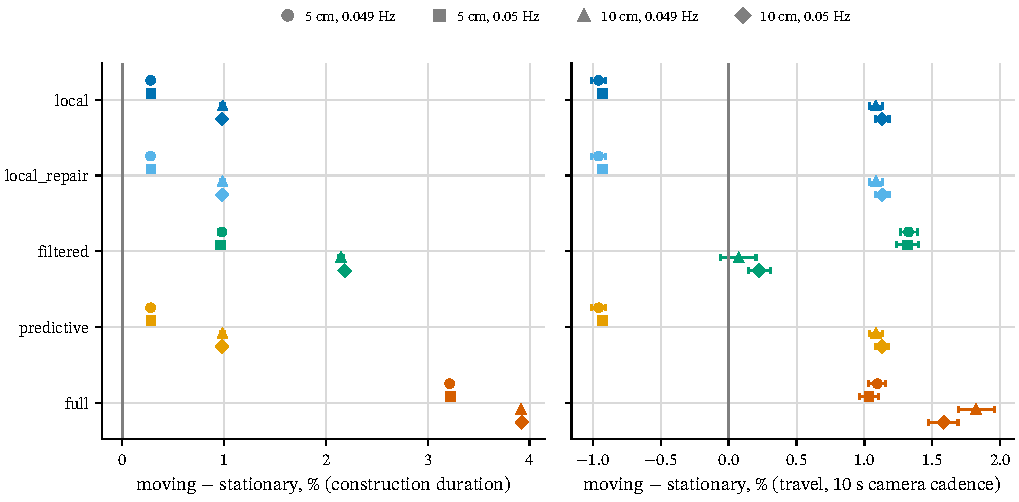
\includegraphics[width=\linewidth]{figures/mulder/v3_paired_effects}
\caption{Model v3 tracking: paired moving-minus-stationary percentage change in construction time (left) and
10\,s-sampled travel (right) for the five completing policies in all four moving conditions; 95\%
paired-bootstrap intervals (often narrower than the markers); 30 pairs per point. Source:
\texttt{mulder\_\allowbreak{}results/\allowbreak{}paper\_\allowbreak{}validation\_\allowbreak{}v3/\allowbreak{}comparisons.csv}.}
\label{fig:mulder-v3-paired}
\end{figure}

\begin{figure}[htbp]
\centering
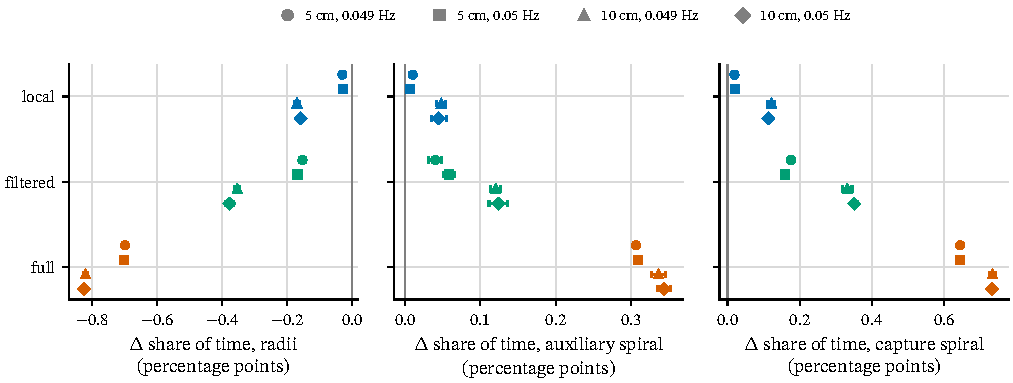
\includegraphics[width=\linewidth]{figures/mulder/v3_phase_allocation}
\caption{Model v3 tracking: paired change in each phase's share of total construction time (percentage
points; stationary shares 38.30\% radii, 12.57\% auxiliary, 37.93\% capture, remainder frame), 95\%
paired-bootstrap intervals, 30 pairs per point. \texttt{local\_\allowbreak{}repair} and \texttt{predictive} equal
\texttt{local}. Source: \texttt{mulder\_\allowbreak{}results/\allowbreak{}paper\_\allowbreak{}validation\_\allowbreak{}v3/\allowbreak{}comparisons.csv}.}
\label{fig:mulder-v3-phase}
\end{figure}

\paragraph{The cost of more planning (C07, C08).} The distributions in
Figure~\ref{fig:mulder-v3-costs} show where the extra time of the proactive policies comes from. At 10\,cm
and 0.05\,Hz \texttt{full} refreshed at every one of the 217 action boundaries after the first, made 218
planning calls and 2{,}095 HTN method calls per trial (against 1 and 32 for \texttt{local}) and spent on
average 1.10\,s of planning wall time against 0.008\,s; \texttt{filtered} made on average 88.1 component
refreshes. Each refresh costs the configured 0.2\,s delay, which accounts for the longer durations; none
improved completion, which was already 30/30 for \texttt{local}. Predictive monitoring cost 1.4\,ms of
prediction time per trial and changed nothing. Hence, in this primary ideal-tracking comparison,
predictive repair did not outperform local feedback (C07) and more frequent full replanning added delay
and planning work without improving completion (C08).

\begin{figure}[htbp]
\centering
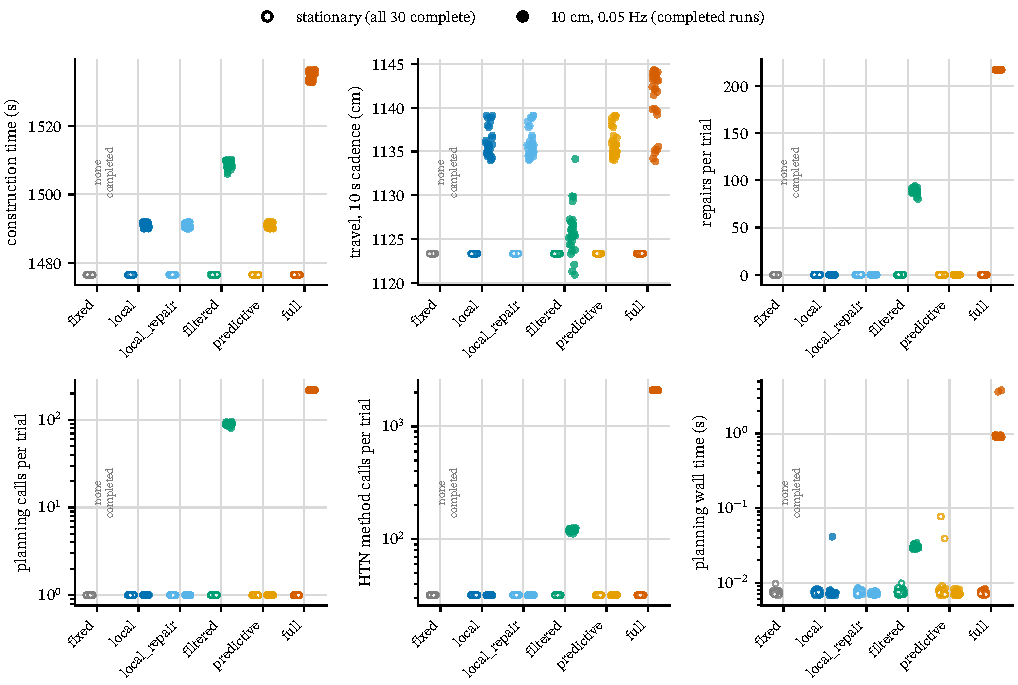
\includegraphics[width=\linewidth]{figures/mulder/v3_cost_distributions}
\caption{Model v3 tracking: per-trial outcomes by policy, stationary runs (open, all 30 complete) and
completed moving runs at 10\,cm, 0.05\,Hz (filled; 30 per policy, none for \texttt{fixed}). Planning calls,
method calls and planning wall time on log scales. Wall time is measured wall-clock time and varies between runs;
all other outcomes are deterministic given the seed. Source:
\texttt{mulder\_\allowbreak{}results/\allowbreak{}paper\_\allowbreak{}validation\_\allowbreak{}v3/\allowbreak{}trials.csv}.}
\label{fig:mulder-v3-costs}
\end{figure}

\paragraph{Sensitivity profiles.} Figure~\ref{fig:mulder-v3-sensitivity} summarises the ten profiles. Halving
the step, halving or doubling speed, tightening the tolerance to 0.1\,cm and a 1\,s repair delay all left
completion at 12/12 and the duration increase between 0.90 and 1.01\%. Duration changes are relative to
each profile's own stationary control, because speed profiles differ in absolute cost (2{,}844.2\,s
stationary at 0.5\,cm/s, 792.8\,s at 2\,cm/s).

\begin{figure}[htbp]
\centering
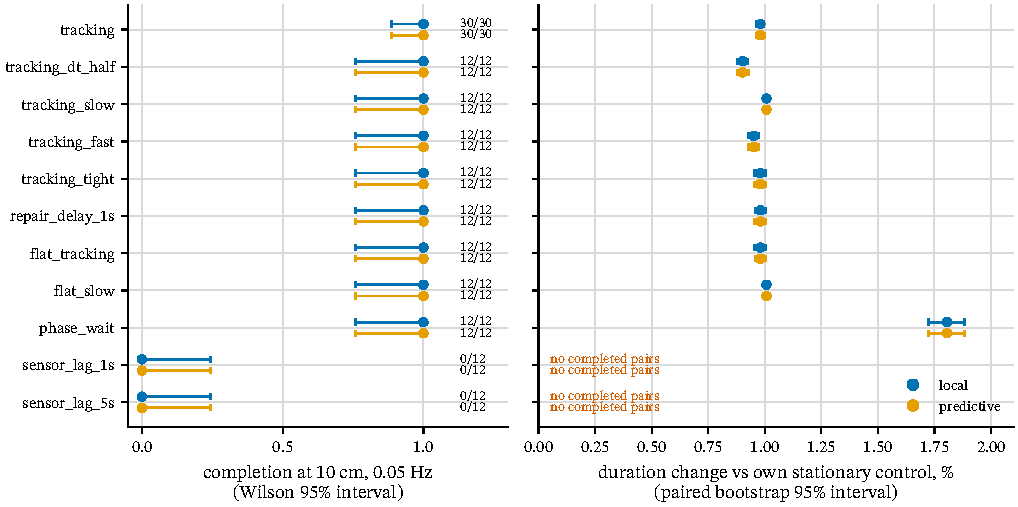
\includegraphics[width=\linewidth]{figures/mulder/v3_sensitivity}
\caption{Model v3 sensitivity and ablation profiles at 10\,cm, 0.05\,Hz for \texttt{local} and \texttt{predictive}.
Left: completion with Wilson 95\% intervals ($n=30$ for \texttt{tracking}, $n=12$ otherwise). Right: paired
duration change against the profile's own stationary control with 95\% paired-bootstrap intervals; the lag
profiles have no completed pairs. Source: \texttt{mulder\_\allowbreak{}results/\allowbreak{}paper\_\allowbreak{}validation\_\allowbreak{}v3/\allowbreak{}trials.csv},
\texttt{comparisons.csv}.}
\label{fig:mulder-v3-sensitivity}
\end{figure}

\paragraph{Sensory lag (C10).} Completion collapsed as soon as sensing was delayed: with a first-order lag
of 1\,s or 5\,s both policies completed 0/12 moving trials (Wilson $[0,0.2425]$), against 12/12 for the
same seeds without lag (Figure~\ref{fig:mulder-lag}). With 1\,s lag \texttt{local} stopped at 2--5 actions and
\texttt{predictive} reached at most 26; with 5\,s lag every trial stopped at 2 actions, three of them at the
120\,s action deadline. Stationary controls with lag completed 12/12. The result contradicts robustness to
substantial sensory lag in the tested profiles; ideal sensing is an important limitation, and the lag
values are assumptions rather than measured spider latencies.

\begin{figure}[htbp]
\centering
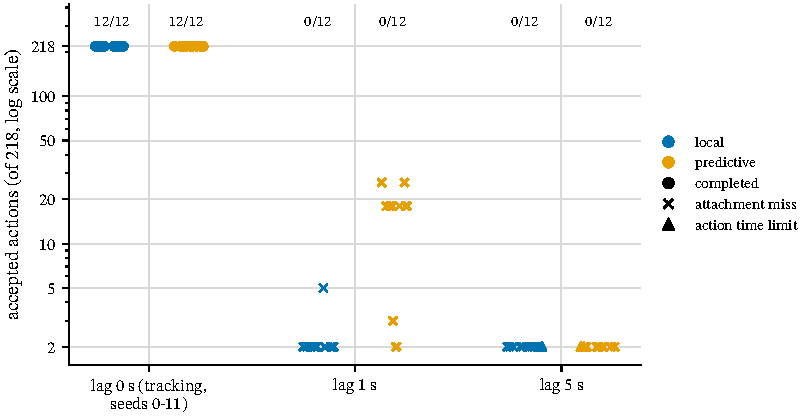
\includegraphics[width=0.85\linewidth]{figures/mulder/v3_sensor_lag}
\caption{Model v3, 10\,cm, 0.05\,Hz: accepted actions per trial with ideal sensing (\texttt{tracking}, seeds 0--11)
and with 1\,s and 5\,s first-order sensory lag; marker shape gives the outcome. Completions above each group.
$n=12$ per policy and lag. Source: \texttt{mulder\_\allowbreak{}results/\allowbreak{}paper\_\allowbreak{}validation\_\allowbreak{}v3/\allowbreak{}trials.csv}.}
\label{fig:mulder-lag}
\end{figure}

\paragraph{Hierarchy ablation (C06).} The flat execution of the same prescribed segment sequence matched the
HTN execution exactly: on all 12 matched moving seeds the duration difference was 0.000000\,s for both
\texttt{local} and \texttt{predictive}, and the moving-minus-stationary change was 0.980\% in both
(Figure~\ref{fig:mulder-flat}). The flat runner makes no compound-method calls (0 against 32). The HTN
hierarchy therefore did not improve disturbance tolerance over the flat baseline in the tested phases;
the supplied sequence plus feedback suffices in this benchmark.

\begin{figure}[htbp]
\centering
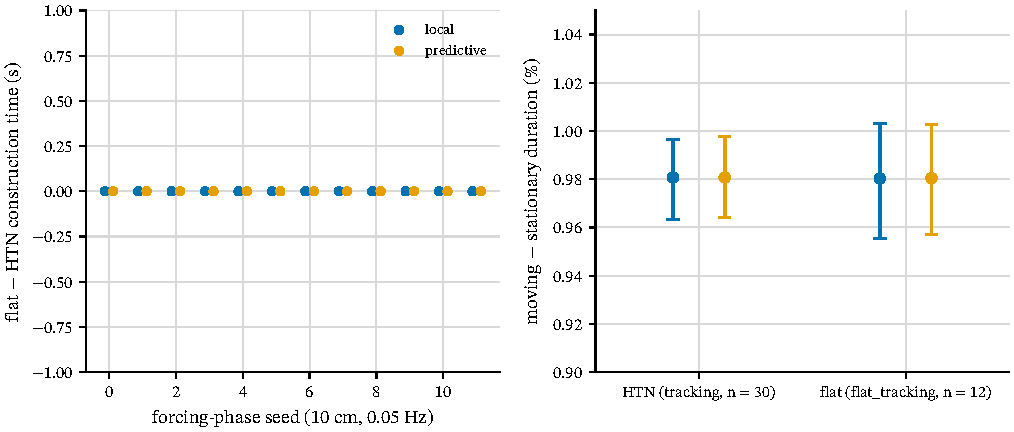
\includegraphics[width=\linewidth]{figures/mulder/v3_flat_vs_htn}
\caption{Model v3 hierarchy ablation at 10\,cm, 0.05\,Hz. Left: per-seed difference in construction time,
\texttt{flat\_\allowbreak{}tracking} minus \texttt{tracking} (12 matched seeds; all exactly zero). Right: paired
moving-minus-stationary duration change with 95\% bootstrap intervals for HTN (30 pairs) and flat (12 pairs).
Source: \texttt{mulder\_\allowbreak{}results/\allowbreak{}paper\_\allowbreak{}validation\_\allowbreak{}v3/\allowbreak{}trials.csv}, \texttt{comparisons.csv}.}
\label{fig:mulder-flat}
\end{figure}

\paragraph{Alternative method: phase\_wait (C11).} The waiting method was chosen 6 or 7 times in every moving
trial (6 in five trials, 7 in seven) and never in stationary runs. On the 12 matched moving seeds it was
slower than \texttt{tracking\_\allowbreak{}slow} by a mean of 22.703291\,s, of which 22.5625\,s was the waiting itself;
the movement it was meant to save was not saved (Figure~\ref{fig:mulder-phase-wait}). Its moving-minus-stationary
cost was 51.36\,s (95\% interval 49.02--53.45\,s), against 28.66\,s for both \texttt{tracking\_\allowbreak{}slow} and
\texttt{flat\_\allowbreak{}slow}. We retain this as an alternative-method negative result.

\begin{figure}[htbp]
\centering
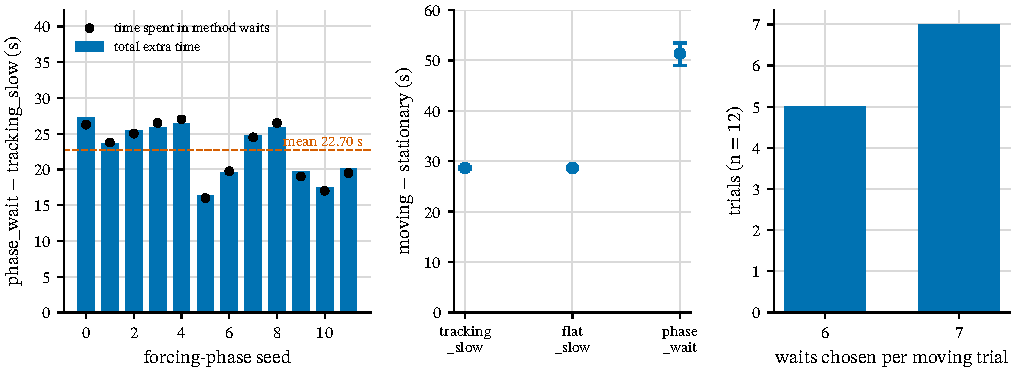
\includegraphics[width=\linewidth]{figures/mulder/v3_phase_wait}
\caption{Model v3 \texttt{phase\_\allowbreak{}wait} (0.5\,cm/s), \texttt{local} policy, 10\,cm, 0.05\,Hz. Left: per-seed construction
time minus the matched \texttt{tracking\_\allowbreak{}slow} run (bars) and time spent in method waits (dots); 12 seeds.
Middle: moving-minus-stationary duration with 95\% paired-bootstrap intervals for the three slow profiles.
Right: number of waits chosen per moving trial. \texttt{predictive} is identical. Source:
\texttt{mulder\_\allowbreak{}results/\allowbreak{}paper\_\allowbreak{}validation\_\allowbreak{}v3/\allowbreak{}trials.csv}, \texttt{comparisons.csv}.}
\label{fig:mulder-phase-wait}
\end{figure}

\paragraph{Measurements against the paper reference (C09, C12).} The repository's
\texttt{paper\_\allowbreak{}reference.json} records the apparatus, the 10\,s sampling interval, the sample sizes (e.g.\ 15
rigid and 9 moving builds for timing, 11 and 9 for geometry) and the published $p$-values of the
rigid--moving comparisons; it contains no per-spider observations and no group means, and no values were
digitised from the paper's plots. The only possible comparison is therefore qualitative, and
Figure~\ref{fig:mulder-paper} sets the model's paired differences beside the paper's $p$-values. The geometric
quantities are identical between moving and stationary runs to within $10^{-12}$: web area
900\,cm$^2$, capture-spiral area 558.615\,cm$^2$, eccentricity 0 (to rounding), 8.5 capture-spiral
crossings, mean mesh space 1.3125\,cm and 16 radii in every completed web. These values are
\emph{imposed}: the counts are prescribed, zero-lag tracking places every end point exactly at its
material target, and the affine shear preserves area. The agreement with the paper's non-significant
geometry results (all six geometry $p$-values, 0.02--0.98, lie above the paper's own threshold of 0.008)
carries no evidential weight. Geometry invariance does not validate the biological
findings (C09), and the simulator is not quantitatively calibrated against the original cohort (C12): the
calibration file reads ``not empirically calibrated: raw observations unavailable''. The rigid-only
fitting and held-out comparison code exists, with an import template, but has not been run on real data.

\begin{figure}[tb]
\centering
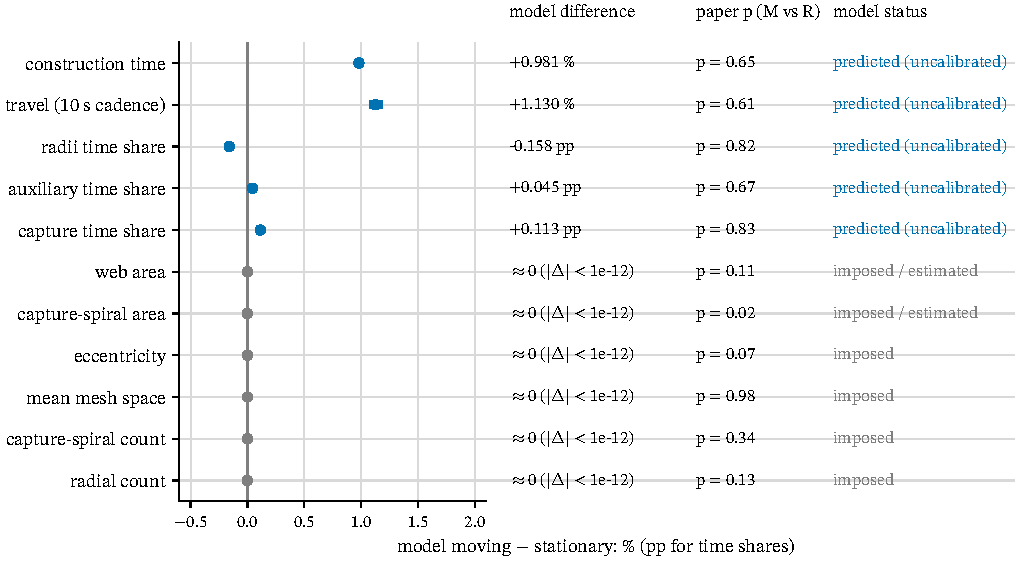
\includegraphics[width=\linewidth]{figures/mulder/v3_geometry_vs_paper}
\caption{Model v3 (\texttt{local}, tracking, 10\,cm, 0.05\,Hz, 30 pairs) paired moving-minus-stationary differences
for the eleven quantities for which Mulder et~al.\ report a rigid-versus-moving $p$-value, alongside those
$p$-values (\texttt{spider\_\allowbreak{}web\_\allowbreak{}mulder/\allowbreak{}paper\_\allowbreak{}reference.json}) and the status of each model quantity. Grey:
imposed by construction (or an envelope estimate of an imposed geometry); blue: model outputs that depend
on uncalibrated speed, dwell and contact assumptions. No biological means or individual observations are
available in the repository, so this is not a quantitative comparison. Source:
\texttt{mulder\_\allowbreak{}results/\allowbreak{}paper\_\allowbreak{}validation\_\allowbreak{}v3/\allowbreak{}comparisons.csv}.}
\label{fig:mulder-paper}
\end{figure}

\subsubsection{Software verification}
\label{sec:mulder-tests}

The package's own tests live in \texttt{spider\_\allowbreak{}web\_\allowbreak{}mulder/\allowbreak{}tests}
(22 in \texttt{test\_\allowbreak{}experiment.py}, 21 in \texttt{test\_\allowbreak{}diagnostics.py} and 16 in
\texttt{test\_\allowbreak{}validation.py}). They check, among other things, identical
stationary execution across policies, seeded reproducibility, the motion-detection, filter, retry and
timestamp contracts of the audit, exact reproduction of first failures by replay, the measurement formulas
and output protection. We re-ran them in a private clone at commit 61d18d8: \textbf{59 passed}. (The
directory holds a further 18 tests in \texttt{test\_\allowbreak{}reentrant.py} for the later IPyHOP back-end, reported
elsewhere; the work log's totals of 98, 114 and 176 tests also include other packages.)

% ---------------------------------------------------------------------------
\subsection{What the benchmark supports, and what it does not}
\label{sec:mulder-claims}

Table~\ref{tab:mulder-claims} restates the ledger entries for this benchmark in their permitted form.
In short: the benchmark is a working software contribution with reproducible, version-tagged evidence.
Under its stated assumptions, ideal local feedback is sufficient for construction on moving supports, and
none of the richer mechanisms (component repair, filtered or predictive refresh, full replanning, the
compound-task hierarchy itself, or an alternative waiting method) improved on it; several cost more.
Two assumptions carry the positive result: ideal sensing (any tested lag removes it) and no-slip passive
advection. Endpoint-only execution fails, which says something about that executor rather than about HTN
planning. Nothing here validates the biological findings: geometry invariance is built in, the timing
outputs are uncalibrated, the uncertainty unit is a forcing phase rather than an animal, and the original
cohort's data have not been obtained. The strongest question the evidence currently supports is when local
feedback is sufficient for moving-support construction and when broader replanning becomes useful
(\texttt{docs/\allowbreak{}research/\allowbreak{}MULDER\_\allowbreak{}OBJECTIVE\_\allowbreak{}ROADMAP.md}).

\begin{table}[H]
\centering
\small
\begin{tabularx}{\linewidth}{@{}l X l X@{}}
\toprule
ID & Statement & Status & Permitted interpretation \\
\midrule
C01 & Moving-support benchmark with six policies implemented & Implemented (v1--v3) & Software/domain contribution, not identified spider cognition \\
C02 & Endpoint-only execution is fragile in the tested moving conditions & Tested; 0/30 at 10\,cm, 0.05\,Hz (v3) & Failure of that executor and model, not physical impossibility or of HTN generally \\
C03 & Ideal continuous local feedback preserves completion & Tested; 30/30, Wilson 0.8865--1 (v3) & Over initial phases, under no-slip advection and ideal sensing \\
C04 & Moving and stationary construction take identical time & Unsupported & Local duration +0.98\%, interval excludes zero; no replication of the paper's non-significant test \\
C05 & Moving supports cause small simulated cost changes under ideal tracking & Tested (v3) & Effect sizes and uncertainty only; no biological equivalence \\
C06 & HTN hierarchy improves disturbance tolerance over the flat baseline & Not supported (v3) & Supplied sequence plus feedback suffices in this benchmark \\
C07 & Predictive repair outperforms simple local feedback & Not demonstrated (v3) & Monitoring/planning costs and stress conditions must be considered \\
C08 & More frequent full replanning improves performance & Not supported (v3 primary) & Adds delay and planning work without improving completion \\
C09 & Geometry invariance validates Mulder's findings & Unsupported & Counts, targets and ideal geometry are imposed; areas are estimates \\
C10 & Results are robust to substantial sensory lag & Contradicted; 0/12 at 1\,s and 5\,s (v3) & Ideal sensing is a key limitation; lag values are assumptions \\
C11 & \texttt{phase\_\allowbreak{}wait} improves construction cost & Not supported; +22.703291\,s (v3) & Alternative-method negative result \\
C12 & Simulator calibrated against the original cohort & Not established & Import/rigid-only fitting implemented, not performed \\
\bottomrule
\end{tabularx}
\caption{Ledger claims for the moving-support benchmark (\texttt{docs/\allowbreak{}research/\allowbreak{}CLAIMS.md}, last updated
2026-11-12), with the version that provides the evidence.}
\label{tab:mulder-claims}
\end{table}

A final note relates this section to the Checkpoint~2 report. There, the HTN agent's advantage was
measured against a random walker that chooses among applicable primitive actions uniformly at random
(Sections~7.5 and~8 of the Checkpoint~2 report). The moving-support benchmark uses a much stronger flat
baseline, the same prescribed action sequence without compound tasks, and against that baseline the
hierarchy added nothing measurable (C06). The two results are not in conflict, since they use different
domains and baselines, but together they indicate that the earlier advantage should be attributed to
structured action ordering rather than to hierarchical decomposition as such.
